\documentclass[11pt,a4paper]{scrartcl}
% =====================================================================
%  pds-apuntes.tex — Estilo común de apuntes y hojas de ejercicios.
%
%  Uso (desde teoría/Tx/apuntes/ o teoría/Tx/ejercicios/):
%     \documentclass[11pt,a4paper]{scrartcl}   % o scrreprt
%     % =====================================================================
%  pds-apuntes.tex — Estilo común de apuntes y hojas de ejercicios.
%
%  Uso (desde teoría/Tx/apuntes/ o teoría/Tx/ejercicios/):
%     \documentclass[11pt,a4paper]{scrartcl}   % o scrreprt
%     % =====================================================================
%  pds-apuntes.tex — Estilo común de apuntes y hojas de ejercicios.
%
%  Uso (desde teoría/Tx/apuntes/ o teoría/Tx/ejercicios/):
%     \documentclass[11pt,a4paper]{scrartcl}   % o scrreprt
%     \input{../../comun/pds-apuntes}
%     \tema{1}{Introducción: señales y sistemas}
%     \begin{document} \cabecera{Apuntes} ... \end{document}
%  Compilar con:  latexmk -xelatex  (o «make» desde teoría/)
% =====================================================================

\input{../../comun/pds-comun.tex}

\usepackage[a4paper, top=2.6cm, bottom=2.6cm, left=2.5cm, right=2.5cm,
            headheight=1.1cm]{geometry}
\usepackage{fontspec}
\usepackage{unicode-math}
\setmainfont{LibertinusSerif}[Extension=.otf, UprightFont=*-Regular, BoldFont=*-Semibold,
  ItalicFont=*-Italic, BoldItalicFont=*-SemiboldItalic]
\setsansfont{FiraSans}[Extension=.otf, UprightFont=*-Regular, BoldFont=*-SemiBold,
  ItalicFont=*-Italic, BoldItalicFont=*-SemiBoldItalic, Scale=MatchLowercase]
\setmonofont{FiraMono}[Extension=.otf, UprightFont=*-Regular, BoldFont=*-Medium, AutoFakeSlant=0.15, Scale=0.85]
\setmathfont{LibertinusMath-Regular.otf}

\usepackage{microtype}
\usepackage{enumitem}
\usepackage{multicol}
\setlist{itemsep=2pt, topsep=4pt}
\usepackage{caption}
\captionsetup{font=small, labelfont={sf,bf,color=pdsazul}, labelsep=period}
\usepackage{subcaption}
\usepackage[most]{tcolorbox}
\usepackage{environ}
\usepackage{scrlayer-scrpage}
\usepackage[hidelinks, unicode]{hyperref}
\usepackage[spanish, noabbrev]{cleveref}

% Títulos en Fira Sans con el azul de la asignatura
\setkomafont{disposition}{\sffamily\bfseries\color{pdsazul}}
\setkomafont{descriptionlabel}{\sffamily\bfseries}
\setlength{\parindent}{0pt}
\setlength{\parskip}{0.55\baselineskip plus 2pt}
\linespread{1.05}

% ---------------------------------------------------------------------
%  Datos del tema y cabeceras
% ---------------------------------------------------------------------
\newcommand{\numtema}{}
\newcommand{\nombretema}{}
\newcommand{\tema}[2]{\renewcommand{\numtema}{#1}\renewcommand{\nombretema}{#2}}

\pagestyle{scrheadings}
\clearpairofpagestyles
\ihead{\sffamily\small\color{pdsgris}\asignatura}
\ohead{\sffamily\small\color{pdsgris}Tema~\numtema. \nombretema}
\ifoot{\sffamily\small\color{pdsgris}\grado}
\ofoot{\sffamily\small\pagemark}
\setkomafont{pagehead}{\normalfont}
\setkomafont{pagefoot}{\normalfont}

% \cabecera{Apuntes|Ejercicios|...} : bloque de título de la primera página
\newcommand{\cabecera}[1]{%
  \thispagestyle{plain.scrheadings}%
  \noindent
  \begin{minipage}[c]{2.2cm}
    
\includegraphics[width=1.9cm]{../../comun/ucm.png}
  \end{minipage}%
  \begin{minipage}[c]{\dimexpr\linewidth-2.2cm}
    \sffamily
    {\small\color{pdsgris}\grado\par \asignatura\ · \curso\par}
    \vspace{4pt}
    {\Large\bfseries\color{pdsazul}#1\par}
    {\large\bfseries Tema~\numtema. \nombretema\par}
    \vspace{2pt}
    {\small\color{pdsgris}\autores\par}
  \end{minipage}\par
  \vspace{6pt}{\color{pdsazul}\rule{\linewidth}{0.8pt}}\par\vspace{4pt}}

% ---------------------------------------------------------------------
%  Cajas: definición, propiedad, ejemplo, nota, «en código»
% ---------------------------------------------------------------------
\tcbset{pdsbase/.style={enhanced, breakable, boxrule=0pt, arc=1.5pt, left=8pt, right=8pt,
    top=5pt, bottom=5pt, fonttitle=\sffamily\bfseries\small, coltitle=white,
    before skip=8pt, after skip=8pt}}
\newtcbtheorem[number within=section]{definicion}{Definición}%
  {pdsbase, colback=pdsfondo, colframe=pdsazul, borderline west={2.5pt}{0pt}{pdsazul}}{def}
\newtcbtheorem[use counter from=definicion]{propiedad}{Propiedad}%
  {pdsbase, colback=pdsfondo, colframe=pdsazul!75, borderline west={2.5pt}{0pt}{pdsazul!75}}{prop}
\newtcbtheorem[use counter from=definicion]{ejemplo}{Ejemplo}%
  {pdsbase, colback=pdsverde!5, colframe=pdsverde, borderline west={2.5pt}{0pt}{pdsverde}}{ej}
\newtcolorbox{nota}[1][Nota]{pdsbase, colback=pdsnaranja!7, colframe=pdsnaranja,
  title={#1}, borderline west={2.5pt}{0pt}{pdsnaranja}}
\newtcolorbox{importante}[1][Importante]{pdsbase, colback=pdsrojo!5, colframe=pdsrojo,
  title={#1}, borderline west={2.5pt}{0pt}{pdsrojo}}
\newtcolorbox{encodigo}[1][En código]{pdsbase, colback=white, colframe=pdsgris,
  title={#1}, borderline west={2.5pt}{0pt}{pdsgris}}

\lstset{basicstyle=\ttfamily\small}
\renewcommand{\codigoetiqueta}[1]{{\sffamily\small\bfseries\color{pdsgris}#1}}

% ---------------------------------------------------------------------
%  Hojas de ejercicios: \begin{ejercicio} ... \end{ejercicio} y
%  \begin{solucion} ... \end{solucion} (solo se imprime si se define
%  \SOLUCIONES antes de cargar el documento; ver *-Soluciones.tex)
% ---------------------------------------------------------------------
\newif\ifsoluciones
\ifdefined\SOLUCIONES \solucionestrue \fi
\newcounter{ejercicio}
\newenvironment{ejercicio}[1][]{%
  \refstepcounter{ejercicio}\par\vspace{6pt}%
  \noindent{\sffamily\bfseries\color{pdsazul}Ejercicio~\theejercicio}%
  \if\relax\detokenize{#1}\relax\else\ {\sffamily\color{pdsgris}(#1)}\fi\quad}%
  {\par}
\NewEnviron{solucion}{%
  \ifsoluciones
    \begin{tcolorbox}[pdsbase, colback=pdsverde!4, colframe=pdsverde,
      borderline west={2.5pt}{0pt}{pdsverde}, title={Solución}]
      \BODY
    \end{tcolorbox}
  \fi}
% \begin{incisos}[columnas] ... \end{incisos}: apartados a), b)... de un
% enunciado repartidos en columnas (3 por defecto)
% (con una sola columna no se usa multicols, que necesita al menos dos)
\newenvironment{incisos}[1][3]{\par\vspace{-2pt}%
  \ifnum#1>1 \def\finincisos{\end{multicols}}\begin{multicols}{#1}\raggedcolumns\raggedright
  \else\def\finincisos{}\fi
  \begin{enumerate}[label=\alph*), itemsep=3pt, topsep=0pt]}%
  {\end{enumerate}\finincisos\vspace{-4pt}}
\newcommand{\herramienta}[1]{\emph{Herramienta interactiva:} \texttt{herramientas/#1}}

%     \tema{1}{Introducción: señales y sistemas}
%     \begin{document} \cabecera{Apuntes} ... \end{document}
%  Compilar con:  latexmk -xelatex  (o «make» desde teoría/)
% =====================================================================

% =====================================================================
%  pds-comun.tex — Paquetes, colores y estilos de código comunes a
%  transparencias, apuntes y hojas de ejercicios. Compilar con XeLaTeX.
%  No cargar directamente: lo cargan pds-beamer.tex y pds-apuntes.tex.
% =====================================================================

\usepackage{polyglossia}
\setmainlanguage{spanish}
\usepackage{mathtools}
\usepackage{graphicx}
\usepackage{booktabs}
\usepackage{multirow}
\usepackage{array}
\usepackage{xcolor}
\usepackage{tikz}
\usetikzlibrary{positioning,arrows.meta,calc,shapes.geometric,decorations.pathreplacing}
\usepackage{listings}
\usepackage{siunitx}
\sisetup{output-decimal-marker={,}, group-separator={\,}, per-mode=symbol}

% Notas de erratas de versiones anteriores: no se imprimen salvo que se
% defina \ERRATAS antes de cargar el estilo (make ERRATAS=1)
\newif\iferratas
\ifdefined\ERRATAS \erratastrue \fi

% Ruta común (logo y figuras compartidas)
\providecommand{\rutacomun}{../../comun/}
\input{\rutacomun datos.tex}

% ---------------------------------------------------------------------
%  Paleta (la misma que usan las figuras generadas con Python,
%  ver comun/pds_estilo.py)
% ---------------------------------------------------------------------
\definecolor{pdsazul}{HTML}{2B3A8C}
\definecolor{pdsrojo}{HTML}{C0392B}
\definecolor{pdsverde}{HTML}{1E7B4F}
\definecolor{pdsnaranja}{HTML}{D9822B}
\definecolor{pdsgris}{HTML}{5A5A66}
\definecolor{pdsfondo}{HTML}{F3F4FA}
\definecolor{pdscodigo}{HTML}{F7F7F2}

% ---------------------------------------------------------------------
%  Diagramas de bloques (TikZ)
% ---------------------------------------------------------------------
\tikzset{
  bloque/.style={rectangle, rounded corners=2pt, draw=pdsazul!80, fill=pdsfondo,
                 very thick, minimum height=8mm, minimum width=14mm, align=center},
  sumador/.style={circle, draw=pdsazul!80, fill=pdsfondo, thick, inner sep=1.5pt},
  flecha/.style={-{Stealth[length=2.2mm]}, thick, pdsgris},
}

% ---------------------------------------------------------------------
%  Código: Python y Matlab en paralelo
% ---------------------------------------------------------------------
\newcommand{\pdscodesize}{\footnotesize}
\lstdefinestyle{pds}{
  basicstyle=\ttfamily\pdscodesize,
  keywordstyle=\color{pdsazul}\bfseries,
  commentstyle=\color{pdsverde}\itshape,
  stringstyle=\color{pdsrojo},
  numbers=none,
  backgroundcolor=\color{pdscodigo},
  frame=single, rulecolor=\color{pdsgris!40}, framerule=0.4pt,
  xleftmargin=2pt, xrightmargin=2pt, aboveskip=2pt, belowskip=2pt,
  columns=fullflexible, keepspaces=true,
  showstringspaces=false, breaklines=true, tabsize=4,
  upquote=true,
  % Con XeLaTeX, listings desordena los caracteres no ASCII junto a
  % dígitos («2π» sale «π2»): se sustituyen por su versión matemática.
  literate={π}{{$\pi$}}1 {δ}{{$\delta$}}1 {ω}{{$\omega$}}1 {Ω}{{$\Omega$}}1
           {≈}{{$\approx$}}1 {µ}{{$\mu$}}1 {·}{{$\cdot$}}1 {α}{{$\alpha$}}1
           {á}{{á}}1 {é}{{é}}1 {í}{{í}}1 {ó}{{ó}}1 {ú}{{ú}}1 {ñ}{{ñ}}1 {¿}{{¿}}1,
}
\lstdefinestyle{python}{style=pds, language=Python,
  morekeywords={as,True,False,None}}
\lstdefinestyle{matlab}{style=pds, language=Matlab,
  morekeywords={function,end,true,false}}

% \codigo{<ruta sin extensión>} muestra el mismo ejemplo en Python
% y en Matlab, uno al lado del otro. Los ficheros viven en
% ../codigo/python/<nombre>.py y ../codigo/matlab/<nombre>.m y se
% ejecutan en las pruebas (make prueba-codigo).
\newcommand{\rutacodigo}{../codigo/}
\newcommand{\codigoetiqueta}[1]{{\sffamily\scriptsize\bfseries\color{pdsgris}#1}}
\newcommand{\codigo}[2][]{%
  \par\noindent
  \begin{minipage}[t]{0.495\linewidth}
    \codigoetiqueta{Python}\par\vspace{1pt}
    \lstinputlisting[style=python,#1]{\rutacodigo python/#2.py}
  \end{minipage}\hfill
  \begin{minipage}[t]{0.495\linewidth}
    \codigoetiqueta{Matlab}\par\vspace{1pt}
    \lstinputlisting[style=matlab,#1]{\rutacodigo matlab/#2.m}
  \end{minipage}\par}

\input{\rutacomun notacion.tex}


\usepackage[a4paper, top=2.6cm, bottom=2.6cm, left=2.5cm, right=2.5cm,
            headheight=1.1cm]{geometry}
\usepackage{fontspec}
\usepackage{unicode-math}
\setmainfont{LibertinusSerif}[Extension=.otf, UprightFont=*-Regular, BoldFont=*-Semibold,
  ItalicFont=*-Italic, BoldItalicFont=*-SemiboldItalic]
\setsansfont{FiraSans}[Extension=.otf, UprightFont=*-Regular, BoldFont=*-SemiBold,
  ItalicFont=*-Italic, BoldItalicFont=*-SemiBoldItalic, Scale=MatchLowercase]
\setmonofont{FiraMono}[Extension=.otf, UprightFont=*-Regular, BoldFont=*-Medium, AutoFakeSlant=0.15, Scale=0.85]
\setmathfont{LibertinusMath-Regular.otf}

\usepackage{microtype}
\usepackage{enumitem}
\usepackage{multicol}
\setlist{itemsep=2pt, topsep=4pt}
\usepackage{caption}
\captionsetup{font=small, labelfont={sf,bf,color=pdsazul}, labelsep=period}
\usepackage{subcaption}
\usepackage[most]{tcolorbox}
\usepackage{environ}
\usepackage{scrlayer-scrpage}
\usepackage[hidelinks, unicode]{hyperref}
\usepackage[spanish, noabbrev]{cleveref}

% Títulos en Fira Sans con el azul de la asignatura
\setkomafont{disposition}{\sffamily\bfseries\color{pdsazul}}
\setkomafont{descriptionlabel}{\sffamily\bfseries}
\setlength{\parindent}{0pt}
\setlength{\parskip}{0.55\baselineskip plus 2pt}
\linespread{1.05}

% ---------------------------------------------------------------------
%  Datos del tema y cabeceras
% ---------------------------------------------------------------------
\newcommand{\numtema}{}
\newcommand{\nombretema}{}
\newcommand{\tema}[2]{\renewcommand{\numtema}{#1}\renewcommand{\nombretema}{#2}}

\pagestyle{scrheadings}
\clearpairofpagestyles
\ihead{\sffamily\small\color{pdsgris}\asignatura}
\ohead{\sffamily\small\color{pdsgris}Tema~\numtema. \nombretema}
\ifoot{\sffamily\small\color{pdsgris}\grado}
\ofoot{\sffamily\small\pagemark}
\setkomafont{pagehead}{\normalfont}
\setkomafont{pagefoot}{\normalfont}

% \cabecera{Apuntes|Ejercicios|...} : bloque de título de la primera página
\newcommand{\cabecera}[1]{%
  \thispagestyle{plain.scrheadings}%
  \noindent
  \begin{minipage}[c]{2.2cm}
    
\includegraphics[width=1.9cm]{../../comun/ucm.png}
  \end{minipage}%
  \begin{minipage}[c]{\dimexpr\linewidth-2.2cm}
    \sffamily
    {\small\color{pdsgris}\grado\par \asignatura\ · \curso\par}
    \vspace{4pt}
    {\Large\bfseries\color{pdsazul}#1\par}
    {\large\bfseries Tema~\numtema. \nombretema\par}
    \vspace{2pt}
    {\small\color{pdsgris}\autores\par}
  \end{minipage}\par
  \vspace{6pt}{\color{pdsazul}\rule{\linewidth}{0.8pt}}\par\vspace{4pt}}

% ---------------------------------------------------------------------
%  Cajas: definición, propiedad, ejemplo, nota, «en código»
% ---------------------------------------------------------------------
\tcbset{pdsbase/.style={enhanced, breakable, boxrule=0pt, arc=1.5pt, left=8pt, right=8pt,
    top=5pt, bottom=5pt, fonttitle=\sffamily\bfseries\small, coltitle=white,
    before skip=8pt, after skip=8pt}}
\newtcbtheorem[number within=section]{definicion}{Definición}%
  {pdsbase, colback=pdsfondo, colframe=pdsazul, borderline west={2.5pt}{0pt}{pdsazul}}{def}
\newtcbtheorem[use counter from=definicion]{propiedad}{Propiedad}%
  {pdsbase, colback=pdsfondo, colframe=pdsazul!75, borderline west={2.5pt}{0pt}{pdsazul!75}}{prop}
\newtcbtheorem[use counter from=definicion]{ejemplo}{Ejemplo}%
  {pdsbase, colback=pdsverde!5, colframe=pdsverde, borderline west={2.5pt}{0pt}{pdsverde}}{ej}
\newtcolorbox{nota}[1][Nota]{pdsbase, colback=pdsnaranja!7, colframe=pdsnaranja,
  title={#1}, borderline west={2.5pt}{0pt}{pdsnaranja}}
\newtcolorbox{importante}[1][Importante]{pdsbase, colback=pdsrojo!5, colframe=pdsrojo,
  title={#1}, borderline west={2.5pt}{0pt}{pdsrojo}}
\newtcolorbox{encodigo}[1][En código]{pdsbase, colback=white, colframe=pdsgris,
  title={#1}, borderline west={2.5pt}{0pt}{pdsgris}}

\lstset{basicstyle=\ttfamily\small}
\renewcommand{\codigoetiqueta}[1]{{\sffamily\small\bfseries\color{pdsgris}#1}}

% ---------------------------------------------------------------------
%  Hojas de ejercicios: \begin{ejercicio} ... \end{ejercicio} y
%  \begin{solucion} ... \end{solucion} (solo se imprime si se define
%  \SOLUCIONES antes de cargar el documento; ver *-Soluciones.tex)
% ---------------------------------------------------------------------
\newif\ifsoluciones
\ifdefined\SOLUCIONES \solucionestrue \fi
\newcounter{ejercicio}
\newenvironment{ejercicio}[1][]{%
  \refstepcounter{ejercicio}\par\vspace{6pt}%
  \noindent{\sffamily\bfseries\color{pdsazul}Ejercicio~\theejercicio}%
  \if\relax\detokenize{#1}\relax\else\ {\sffamily\color{pdsgris}(#1)}\fi\quad}%
  {\par}
\NewEnviron{solucion}{%
  \ifsoluciones
    \begin{tcolorbox}[pdsbase, colback=pdsverde!4, colframe=pdsverde,
      borderline west={2.5pt}{0pt}{pdsverde}, title={Solución}]
      \BODY
    \end{tcolorbox}
  \fi}
% \begin{incisos}[columnas] ... \end{incisos}: apartados a), b)... de un
% enunciado repartidos en columnas (3 por defecto)
% (con una sola columna no se usa multicols, que necesita al menos dos)
\newenvironment{incisos}[1][3]{\par\vspace{-2pt}%
  \ifnum#1>1 \def\finincisos{\end{multicols}}\begin{multicols}{#1}\raggedcolumns\raggedright
  \else\def\finincisos{}\fi
  \begin{enumerate}[label=\alph*), itemsep=3pt, topsep=0pt]}%
  {\end{enumerate}\finincisos\vspace{-4pt}}
\newcommand{\herramienta}[1]{\emph{Herramienta interactiva:} \texttt{herramientas/#1}}

%     \tema{1}{Introducción: señales y sistemas}
%     \begin{document} \cabecera{Apuntes} ... \end{document}
%  Compilar con:  latexmk -xelatex  (o «make» desde teoría/)
% =====================================================================

% =====================================================================
%  pds-comun.tex — Paquetes, colores y estilos de código comunes a
%  transparencias, apuntes y hojas de ejercicios. Compilar con XeLaTeX.
%  No cargar directamente: lo cargan pds-beamer.tex y pds-apuntes.tex.
% =====================================================================

\usepackage{polyglossia}
\setmainlanguage{spanish}
\usepackage{mathtools}
\usepackage{graphicx}
\usepackage{booktabs}
\usepackage{multirow}
\usepackage{array}
\usepackage{xcolor}
\usepackage{tikz}
\usetikzlibrary{positioning,arrows.meta,calc,shapes.geometric,decorations.pathreplacing}
\usepackage{listings}
\usepackage{siunitx}
\sisetup{output-decimal-marker={,}, group-separator={\,}, per-mode=symbol}

% Notas de erratas de versiones anteriores: no se imprimen salvo que se
% defina \ERRATAS antes de cargar el estilo (make ERRATAS=1)
\newif\iferratas
\ifdefined\ERRATAS \erratastrue \fi

% Ruta común (logo y figuras compartidas)
\providecommand{\rutacomun}{../../comun/}
\input{\rutacomun datos.tex}

% ---------------------------------------------------------------------
%  Paleta (la misma que usan las figuras generadas con Python,
%  ver comun/pds_estilo.py)
% ---------------------------------------------------------------------
\definecolor{pdsazul}{HTML}{2B3A8C}
\definecolor{pdsrojo}{HTML}{C0392B}
\definecolor{pdsverde}{HTML}{1E7B4F}
\definecolor{pdsnaranja}{HTML}{D9822B}
\definecolor{pdsgris}{HTML}{5A5A66}
\definecolor{pdsfondo}{HTML}{F3F4FA}
\definecolor{pdscodigo}{HTML}{F7F7F2}

% ---------------------------------------------------------------------
%  Diagramas de bloques (TikZ)
% ---------------------------------------------------------------------
\tikzset{
  bloque/.style={rectangle, rounded corners=2pt, draw=pdsazul!80, fill=pdsfondo,
                 very thick, minimum height=8mm, minimum width=14mm, align=center},
  sumador/.style={circle, draw=pdsazul!80, fill=pdsfondo, thick, inner sep=1.5pt},
  flecha/.style={-{Stealth[length=2.2mm]}, thick, pdsgris},
}

% ---------------------------------------------------------------------
%  Código: Python y Matlab en paralelo
% ---------------------------------------------------------------------
\newcommand{\pdscodesize}{\footnotesize}
\lstdefinestyle{pds}{
  basicstyle=\ttfamily\pdscodesize,
  keywordstyle=\color{pdsazul}\bfseries,
  commentstyle=\color{pdsverde}\itshape,
  stringstyle=\color{pdsrojo},
  numbers=none,
  backgroundcolor=\color{pdscodigo},
  frame=single, rulecolor=\color{pdsgris!40}, framerule=0.4pt,
  xleftmargin=2pt, xrightmargin=2pt, aboveskip=2pt, belowskip=2pt,
  columns=fullflexible, keepspaces=true,
  showstringspaces=false, breaklines=true, tabsize=4,
  upquote=true,
  % Con XeLaTeX, listings desordena los caracteres no ASCII junto a
  % dígitos («2π» sale «π2»): se sustituyen por su versión matemática.
  literate={π}{{$\pi$}}1 {δ}{{$\delta$}}1 {ω}{{$\omega$}}1 {Ω}{{$\Omega$}}1
           {≈}{{$\approx$}}1 {µ}{{$\mu$}}1 {·}{{$\cdot$}}1 {α}{{$\alpha$}}1
           {á}{{á}}1 {é}{{é}}1 {í}{{í}}1 {ó}{{ó}}1 {ú}{{ú}}1 {ñ}{{ñ}}1 {¿}{{¿}}1,
}
\lstdefinestyle{python}{style=pds, language=Python,
  morekeywords={as,True,False,None}}
\lstdefinestyle{matlab}{style=pds, language=Matlab,
  morekeywords={function,end,true,false}}

% \codigo{<ruta sin extensión>} muestra el mismo ejemplo en Python
% y en Matlab, uno al lado del otro. Los ficheros viven en
% ../codigo/python/<nombre>.py y ../codigo/matlab/<nombre>.m y se
% ejecutan en las pruebas (make prueba-codigo).
\newcommand{\rutacodigo}{../codigo/}
\newcommand{\codigoetiqueta}[1]{{\sffamily\scriptsize\bfseries\color{pdsgris}#1}}
\newcommand{\codigo}[2][]{%
  \par\noindent
  \begin{minipage}[t]{0.495\linewidth}
    \codigoetiqueta{Python}\par\vspace{1pt}
    \lstinputlisting[style=python,#1]{\rutacodigo python/#2.py}
  \end{minipage}\hfill
  \begin{minipage}[t]{0.495\linewidth}
    \codigoetiqueta{Matlab}\par\vspace{1pt}
    \lstinputlisting[style=matlab,#1]{\rutacodigo matlab/#2.m}
  \end{minipage}\par}

\input{\rutacomun notacion.tex}


\usepackage[a4paper, top=2.6cm, bottom=2.6cm, left=2.5cm, right=2.5cm,
            headheight=1.1cm]{geometry}
\usepackage{fontspec}
\usepackage{unicode-math}
\setmainfont{LibertinusSerif}[Extension=.otf, UprightFont=*-Regular, BoldFont=*-Semibold,
  ItalicFont=*-Italic, BoldItalicFont=*-SemiboldItalic]
\setsansfont{FiraSans}[Extension=.otf, UprightFont=*-Regular, BoldFont=*-SemiBold,
  ItalicFont=*-Italic, BoldItalicFont=*-SemiBoldItalic, Scale=MatchLowercase]
\setmonofont{FiraMono}[Extension=.otf, UprightFont=*-Regular, BoldFont=*-Medium, AutoFakeSlant=0.15, Scale=0.85]
\setmathfont{LibertinusMath-Regular.otf}

\usepackage{microtype}
\usepackage{enumitem}
\usepackage{multicol}
\setlist{itemsep=2pt, topsep=4pt}
\usepackage{caption}
\captionsetup{font=small, labelfont={sf,bf,color=pdsazul}, labelsep=period}
\usepackage{subcaption}
\usepackage[most]{tcolorbox}
\usepackage{environ}
\usepackage{scrlayer-scrpage}
\usepackage[hidelinks, unicode]{hyperref}
\usepackage[spanish, noabbrev]{cleveref}

% Títulos en Fira Sans con el azul de la asignatura
\setkomafont{disposition}{\sffamily\bfseries\color{pdsazul}}
\setkomafont{descriptionlabel}{\sffamily\bfseries}
\setlength{\parindent}{0pt}
\setlength{\parskip}{0.55\baselineskip plus 2pt}
\linespread{1.05}

% ---------------------------------------------------------------------
%  Datos del tema y cabeceras
% ---------------------------------------------------------------------
\newcommand{\numtema}{}
\newcommand{\nombretema}{}
\newcommand{\tema}[2]{\renewcommand{\numtema}{#1}\renewcommand{\nombretema}{#2}}

\pagestyle{scrheadings}
\clearpairofpagestyles
\ihead{\sffamily\small\color{pdsgris}\asignatura}
\ohead{\sffamily\small\color{pdsgris}Tema~\numtema. \nombretema}
\ifoot{\sffamily\small\color{pdsgris}\grado}
\ofoot{\sffamily\small\pagemark}
\setkomafont{pagehead}{\normalfont}
\setkomafont{pagefoot}{\normalfont}

% \cabecera{Apuntes|Ejercicios|...} : bloque de título de la primera página
\newcommand{\cabecera}[1]{%
  \thispagestyle{plain.scrheadings}%
  \noindent
  \begin{minipage}[c]{2.2cm}
    
\includegraphics[width=1.9cm]{../../comun/ucm.png}
  \end{minipage}%
  \begin{minipage}[c]{\dimexpr\linewidth-2.2cm}
    \sffamily
    {\small\color{pdsgris}\grado\par \asignatura\ · \curso\par}
    \vspace{4pt}
    {\Large\bfseries\color{pdsazul}#1\par}
    {\large\bfseries Tema~\numtema. \nombretema\par}
    \vspace{2pt}
    {\small\color{pdsgris}\autores\par}
  \end{minipage}\par
  \vspace{6pt}{\color{pdsazul}\rule{\linewidth}{0.8pt}}\par\vspace{4pt}}

% ---------------------------------------------------------------------
%  Cajas: definición, propiedad, ejemplo, nota, «en código»
% ---------------------------------------------------------------------
\tcbset{pdsbase/.style={enhanced, breakable, boxrule=0pt, arc=1.5pt, left=8pt, right=8pt,
    top=5pt, bottom=5pt, fonttitle=\sffamily\bfseries\small, coltitle=white,
    before skip=8pt, after skip=8pt}}
\newtcbtheorem[number within=section]{definicion}{Definición}%
  {pdsbase, colback=pdsfondo, colframe=pdsazul, borderline west={2.5pt}{0pt}{pdsazul}}{def}
\newtcbtheorem[use counter from=definicion]{propiedad}{Propiedad}%
  {pdsbase, colback=pdsfondo, colframe=pdsazul!75, borderline west={2.5pt}{0pt}{pdsazul!75}}{prop}
\newtcbtheorem[use counter from=definicion]{ejemplo}{Ejemplo}%
  {pdsbase, colback=pdsverde!5, colframe=pdsverde, borderline west={2.5pt}{0pt}{pdsverde}}{ej}
\newtcolorbox{nota}[1][Nota]{pdsbase, colback=pdsnaranja!7, colframe=pdsnaranja,
  title={#1}, borderline west={2.5pt}{0pt}{pdsnaranja}}
\newtcolorbox{importante}[1][Importante]{pdsbase, colback=pdsrojo!5, colframe=pdsrojo,
  title={#1}, borderline west={2.5pt}{0pt}{pdsrojo}}
\newtcolorbox{encodigo}[1][En código]{pdsbase, colback=white, colframe=pdsgris,
  title={#1}, borderline west={2.5pt}{0pt}{pdsgris}}

\lstset{basicstyle=\ttfamily\small}
\renewcommand{\codigoetiqueta}[1]{{\sffamily\small\bfseries\color{pdsgris}#1}}

% ---------------------------------------------------------------------
%  Hojas de ejercicios: \begin{ejercicio} ... \end{ejercicio} y
%  \begin{solucion} ... \end{solucion} (solo se imprime si se define
%  \SOLUCIONES antes de cargar el documento; ver *-Soluciones.tex)
% ---------------------------------------------------------------------
\newif\ifsoluciones
\ifdefined\SOLUCIONES \solucionestrue \fi
\newcounter{ejercicio}
\newenvironment{ejercicio}[1][]{%
  \refstepcounter{ejercicio}\par\vspace{6pt}%
  \noindent{\sffamily\bfseries\color{pdsazul}Ejercicio~\theejercicio}%
  \if\relax\detokenize{#1}\relax\else\ {\sffamily\color{pdsgris}(#1)}\fi\quad}%
  {\par}
\NewEnviron{solucion}{%
  \ifsoluciones
    \begin{tcolorbox}[pdsbase, colback=pdsverde!4, colframe=pdsverde,
      borderline west={2.5pt}{0pt}{pdsverde}, title={Solución}]
      \BODY
    \end{tcolorbox}
  \fi}
% \begin{incisos}[columnas] ... \end{incisos}: apartados a), b)... de un
% enunciado repartidos en columnas (3 por defecto)
% (con una sola columna no se usa multicols, que necesita al menos dos)
\newenvironment{incisos}[1][3]{\par\vspace{-2pt}%
  \ifnum#1>1 \def\finincisos{\end{multicols}}\begin{multicols}{#1}\raggedcolumns\raggedright
  \else\def\finincisos{}\fi
  \begin{enumerate}[label=\alph*), itemsep=3pt, topsep=0pt]}%
  {\end{enumerate}\finincisos\vspace{-4pt}}
\newcommand{\herramienta}[1]{\emph{Herramienta interactiva:} \texttt{herramientas/#1}}

\graphicspath{{../figuras/}}
\tema{1}{Introducción: señales y sistemas}
\renewcommand{\rutacodigo}{../codigo/}

\hypersetup{pdftitle={Tema 1. Introducción: señales y sistemas},
  pdfauthor={\autores}}

\begin{document}
\cabecera{Apuntes}

\begin{nota}[Cómo usar estos apuntes]
  Estos apuntes desarrollan el contenido de las cuatro presentaciones del tema: las secciones~\ref{sec:intro}–\ref{sec:basicas} corresponden a la parte~1 (tipos de señales y señales básicas), las secciones~\ref{sec:operaciones}–\ref{sec:frecuencia} a la parte~2 (operaciones y análisis en frecuencia), las secciones~\ref{sec:propiedades}–\ref{sec:lti-dc} a la parte~3 (sistemas) y la sección~\ref{sec:aplicaciones} a la parte~4 (señales reales). Los ejemplos de código están en \texttt{teoría/T1/codigo/}, en Python y en Matlab, y se pueden ejecutar tal cual. Al final de cada sección se indican los ejercicios de la hoja del tema que la practican.
\end{nota}

\tableofcontents

% =====================================================================
\section{Señales y sistemas}\label{sec:intro}

El procesamiento de señales estudia cómo representar, analizar y transformar la información que transportan las magnitudes físicas. Este primer tema fija la terminología y repasa las herramientas matemáticas que usaremos durante todo el curso: los tipos de señales, las operaciones que se hacen con ellas, su representación en frecuencia y las propiedades de los sistemas que las transforman. El resultado de aprendizaje que persigue, según la guía docente, es \emph{relacionar señales y sistemas de tiempo continuo con señales y sistemas de tiempo discreto, en el dominio del tiempo y de la frecuencia}. Por eso cada concepto se presenta en sus dos versiones, continua y discreta, señalando dónde se parecen y, sobre todo, dónde se diferencian.

\begin{definicion}{Señal}{senal}
  Una \emph{señal} es una función de una o varias variables independientes (tiempo, espacio, \ldots) que transporta información sobre la evolución de una magnitud física. Ejemplos: la presión acústica que capta un micrófono, la tensión en un electrodo de ECG, la intensidad luminosa de cada punto de una imagen o la temperatura que mide un sensor.
\end{definicion}

\begin{definicion}{Sistema}{sistema}
  Un \emph{sistema} es una entidad que, excitada por una señal de entrada, produce una señal de salida. Modela la transformación que un dispositivo físico (un circuito, un canal de comunicaciones, un sensor) o un algoritmo (un filtro digital, un ecualizador) hace sobre una señal.
\end{definicion}

\subsection{Notación}

A lo largo del curso seguiremos estos convenios, que son los de la bibliografía básica:
\begin{itemize}
  \item Las señales se escriben en minúscula: $x$, $y$, $h$, \ldots{} Una señal de tiempo continuo se escribe $x(t)$, con $t\in\R$; una de tiempo discreto, o \emph{secuencia}, se escribe $x[n]$, con $n\in\Z$. \textbf{Paréntesis para tiempo continuo y corchetes para tiempo discreto}: nunca escribiremos $x(n)$ para una secuencia, porque la diferencia entre ambos tipos de señal es justamente lo que el curso estudia.
  \item Un sistema se representa con un operador $\T$: $y(t)=\sis{x(t)}$ o $y[n]=\sis{x[n]}$.
  \item La frecuencia de una señal continua se escribe $\omega$ (en rad/s) o $f$ (en Hz), con $\omega=2\pi f$. La de una secuencia se escribe $\Omega$ (en rad/muestra) o $F$ (en ciclos/muestra), con $\Omega=2\pi F$. Cuando una secuencia se obtiene muestreando con periodo $T_s$, ambas se relacionan por $\Omega=\omega T_s$ (Tema~2).
  \item Las transformadas se escriben en mayúscula: $\Xc$ (Fourier continua), $\Xd$ (Fourier discreta), $X(s)$ (Laplace), $X(z)$ (Z) y $X[k]$ (DFT, Tema~3).
\end{itemize}

\subsection{Procesado analógico y procesado digital}

Las señales del mundo físico son casi siempre analógicas. Para procesarlas con un computador, un DSP o un microcontrolador se sigue la cadena de la \cref{fig:cadena}: un filtro \emph{antialiasing} limita el ancho de banda, el conversor A/D muestrea y cuantifica, el procesador aplica el algoritmo y, si hace falta devolver una señal analógica, el conversor D/A y el filtro de reconstrucción completan el camino. El Tema~2 estudia el muestreo y la cuantificación; los temas siguientes, el bloque central.

\begin{figure}[ht]
  \centering
  \resizebox{\linewidth}{!}{%
  \begin{tikzpicture}[node distance=0.9cm]
    \node (x) {$x_a(t)$};
    \node[bloque, right=of x] (aa) {Filtro\\antialiasing};
    \node[bloque, right=of aa] (ad) {A/D};
    \node[bloque, right=of ad, fill=pdsazul!12] (dsp) {Procesado\\digital};
    \node[bloque, right=of dsp] (da) {D/A};
    \node[bloque, right=of da] (rec) {Filtro de\\reconstrucción};
    \node[right=of rec] (y) {$y_a(t)$};
    \draw[flecha] (x) -- (aa); \draw[flecha] (aa) -- (ad);
    \draw[flecha] (ad) -- node[above, font=\footnotesize]{$x[n]$} (dsp);
    \draw[flecha] (dsp) -- node[above, font=\footnotesize]{$y[n]$} (da);
    \draw[flecha] (da) -- (rec); \draw[flecha] (rec) -- (y);
  \end{tikzpicture}}
  \caption{Cadena de procesado digital de una señal analógica.}
  \label{fig:cadena}
\end{figure}

El procesado digital tiene ventajas claras: es preciso y repetible (no hay deriva de componentes con la temperatura o el envejecimiento), es flexible (cambiar el algoritmo es cambiar el programa) y permite operaciones muy difíciles en analógico, como filtros de fase lineal, la FFT o los filtros adaptativos. A cambio, el ancho de banda queda limitado por la frecuencia de muestreo, aparecen errores de cuantificación y de precisión finita, y el cálculo introduce retardo y consume energía.

% =====================================================================
\section{Clasificación de las señales}\label{sec:tipos}

\subsection{Dimensión y número de canales}

Una señal es \emph{unidimensional} si depende de una sola variable independiente (normalmente el tiempo) y \emph{multidimensional} si depende de varias: una imagen en escala de grises es una función $x(u,v)$ de dos coordenadas espaciales y un vídeo añade el tiempo, $x(u,v,t)$. Por otro lado, una señal es \emph{escalar} si en cada punto toma un solo valor y \emph{vectorial} (o multicanal) si toma varios: un acelerómetro de tres ejes da $[x_1(t)\ x_2(t)\ x_3(t)]$ y una imagen en color, tres planos $[x_R\ x_G\ x_B](u,v)$. En este curso trabajaremos sobre todo con señales escalares unidimensionales, aunque casi todo se generaliza.

\subsection{Variable independiente y amplitud}

Tanto la variable independiente como la amplitud pueden ser continuas o discretas, lo que da cuatro combinaciones (\cref{fig:analogica}):

\begin{center}
  \begin{tabular}{@{}lll@{}}
    \toprule
    & amplitud continua & amplitud discreta\\\midrule
    tiempo continuo & analógica & cuantificada\\
    tiempo discreto & muestreada & \textbf{digital}\\\bottomrule
  \end{tabular}
\end{center}

Una amplitud discreta toma valores en un conjunto finito o numerable, por ejemplo los múltiplos $k\Delta$ de un escalón de cuantificación. Un computador solo puede representar señales \emph{digitales}, discretas en tiempo y en amplitud. En la mayor parte del curso ignoraremos la cuantificación y trataremos las secuencias como si su amplitud fuera continua; el Tema~2 cuantifica el error que esto supone.

\begin{figure}[ht]
  \centering
  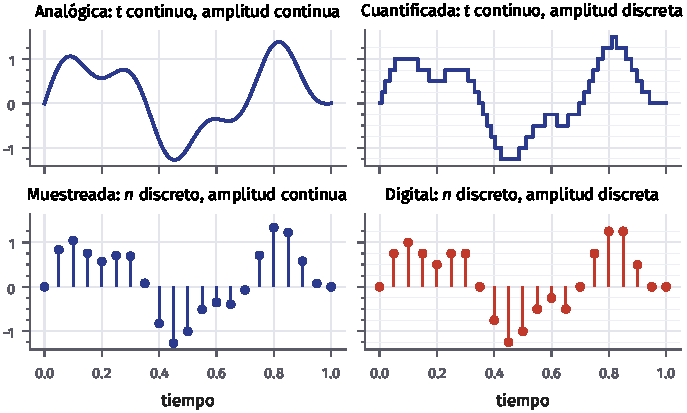
\includegraphics[width=0.75\linewidth]{analogica_digital}
  \caption{Una misma señal analógica, cuantificada, muestreada y digital.}
  \label{fig:analogica}
\end{figure}

\subsection{Deterministas y aleatorias}

Una señal es \emph{determinista} si su valor en cada instante está fijado por una expresión, una tabla o una regla, de modo que se puede predecir. Es \emph{aleatoria} o \emph{estocástica} si su valor en cada instante es una variable aleatoria, y entonces solo se puede describir estadísticamente: con su densidad de probabilidad, su media, su autocorrelación o su densidad espectral de potencia. El ruido de un sensor, la voz o el tráfico de una red se modelan como señales aleatorias; el Tema~6 las estudia con detalle.

\subsection{Periódicas y aperiódicas}

\begin{definicion}{Señal periódica}{periodica}
  Una señal continua es periódica si existe $T>0$ tal que $x(t+T)=x(t)$ para todo $t$. Una secuencia es periódica si existe un entero $N>0$ tal que $x[n+N]=x[n]$ para todo $n$. El menor periodo positivo es el \emph{periodo fundamental}, $T_0$ o $N_0$.
\end{definicion}

Si $T$ es un periodo, también lo es $lT$ para todo entero $l\ne0$: por eso hablamos del periodo \emph{fundamental}. Fíjate en que el periodo de una secuencia tiene que ser entero; esta restricción, que parece inocente, hace que muchas sinusoides discretas no sean periódicas (\cref{sec:exp-discreta}).

La suma de dos señales periódicas continuas, de periodos $T_1$ y $T_2$, es periódica si y solo si el cociente $T_1/T_2$ es racional, $T_1/T_2=p/q$ con $p,q$ enteros primos entre sí. El periodo de la suma es entonces $T_0=qT_1=pT_2$, el mínimo común múltiplo.

\begin{ejemplo}{Suma de sinusoides}{suma}
  $x(t)=\cos(2t)+\cos(3t)$ tiene periodos $T_1=\pi$ y $T_2=2\pi/3$. El cociente $T_1/T_2=3/2$ es racional, así que $x$ es periódica con $T_0=2T_1=3T_2=2\pi$.
  En cambio, $\cos t+\cos(\pi t)$ tiene periodos $2\pi$ y $2$, cuyo cociente $\pi$ es irracional: la suma no es periódica, aunque cada término lo sea.
\end{ejemplo}

\subsection{Pares e impares}

Una señal es \emph{par} si es simétrica respecto al eje vertical, $x(t)=x(-t)$, e \emph{impar} si es simétrica respecto al origen, $x(t)=-x(-t)$; en discreto, igual con $x[n]$. Una señal impar vale necesariamente cero en el origen. El producto de dos señales pares o de dos impares es par, y el de una par por una impar es impar. Además, la integral de una señal impar en un intervalo simétrico es nula, lo que simplifica muchos cálculos de series y transformadas de Fourier.

\begin{propiedad}{Descomposición par–impar}{parimpar}
  Toda señal se escribe de forma única como suma de una parte par y una impar, $x=x_p+x_i$, con
  \[
    x_p(t)=\frac{x(t)+x(-t)}{2},\qquad x_i(t)=\frac{x(t)-x(-t)}{2}.
  \]
\end{propiedad}

Basta comprobar que $x_p$ es par, que $x_i$ es impar y que su suma es $x$. La unicidad se debe a que la única señal que es a la vez par e impar es la nula.

\begin{ejemplo}{Descomposición de una exponencial causal}{parimpar}
  Sea $x[n]=2\,(0{,}8)^n u[n]$. Para $n>0$, $x[-n]=0$, de modo que $x_p[n]=x_i[n]=(0{,}8)^n$; para $n<0$ ocurre lo contrario y $x_p[n]=(0{,}8)^{-n}$, $x_i[n]=-(0{,}8)^{-n}$; y en $n=0$, $x_p[0]=2$, $x_i[0]=0$. En resumen:
  \[
    x_p[n]=\begin{cases}2 & n=0\\ (0{,}8)^{\abs{n}} & n\ne0\end{cases},\qquad
    x_i[n]=\sgn[n]\,(0{,}8)^{\abs{n}}.
  \]
  \centering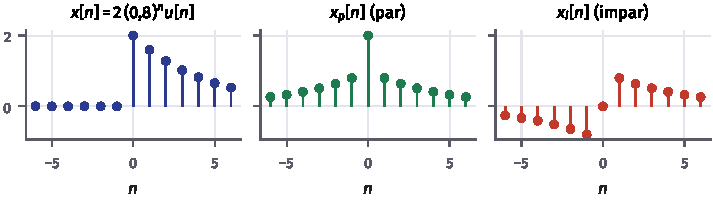
\includegraphics[width=0.85\linewidth]{descomposicion_par_impar}
\end{ejemplo}

\subsection{Causales, anticausales y no causales}

Una señal es \emph{causal} si vale cero para $t<0$ (o $n<0$), \emph{anticausal} si vale cero para $t>0$ (o $n>0$) y \emph{no causal} si no es causal. El nombre procede de los sistemas: la respuesta al impulso de un sistema causal, que es el único que se puede implementar en tiempo real, es una señal causal (\cref{sec:lti}). Multiplicar una señal por el escalón $u(t)$ la hace causal.

\subsection{Señales de energía y de potencia}

\begin{definicion}{Energía y potencia media}{energia}
  \[
    E_x=\int_{-\infty}^{\infty}\abs{x(t)}^2\dd t,\qquad
    P_x=\lim_{T\to\infty}\frac{1}{2T}\int_{-T}^{T}\abs{x(t)}^2\dd t,
  \]
  \[
    E_x=\sum_{n=-\infty}^{\infty}\abs{x[n]}^2,\qquad
    P_x=\lim_{N\to\infty}\frac{1}{2N+1}\sum_{n=-N}^{N}\abs{x[n]}^2.
  \]
\end{definicion}

Si $x$ fuera la tensión sobre una resistencia de \SI{1}{\ohm}, $E_x$ sería la energía disipada y $P_x$ la potencia media; en general las usamos como medidas del «tamaño» de la señal, sin unidades físicas. Una señal es \emph{de energía} si $0<E_x<\infty$, y entonces su potencia es nula, porque la energía acumulada en $[-T,T]$ se mantiene acotada mientras el denominador $2T$ crece. Una señal es \emph{de potencia} si $0<P_x<\infty$, y entonces su energía es infinita. Las señales limitadas en el tiempo o que decaen son de energía; las periódicas, el escalón o un ruido estacionario son de potencia. Algunas señales, como la rampa, no son de ninguno de los dos tipos.

Para una señal periódica basta promediar en un periodo:
\[
  P_x=\frac{1}{T_0}\int_{T_0}\abs{x(t)}^2\dd t,\qquad P_x=\frac{1}{N_0}\sum_{n=0}^{N_0-1}\abs{x[n]}^2.
\]

\begin{ejemplo}{Tres cálculos}{energia}
  \begin{itemize}
    \item $x[n]=a^n u[n]$ con $\abs{a}<1$: por la serie geométrica, $E_x=\sum_{n\ge0}\abs{a}^{2n}=1/(1-\abs{a}^2)$. Es una señal de energía; con $a=0{,}9$, $E_x=5{,}263$.
    \item $x(t)=A\cos(\omega_0t+\phi)$: como $\cos^2\theta=\tfrac12(1+\cos2\theta)$ y el coseno integra cero en un periodo, $P_x=A^2/2$. Es de potencia; con $A=3$, $P_x=4{,}5$.
    \item $u(t)$: su energía es infinita y $P=\lim_{T\to\infty}\frac{1}{2T}\int_0^T\dd t=\tfrac12$.
  \end{itemize}
\end{ejemplo}

\begin{encodigo}
  Aproximamos la suma infinita y el límite con sumas finitas y comparamos con los valores teóricos del ejemplo anterior.
  \codigo{energia_potencia}
\end{encodigo}

\subsection{Señales complejas}

Una señal compleja se describe con dos señales reales, ya sea en forma cartesiana (parte real e imaginaria) o polar (módulo y fase):
\[
  x=\Re\{x\}+j\Im\{x\}=\abs{x}\,\e^{j\arg x},\qquad
  \abs{x}=\sqrt{\Re\{x\}^2+\Im\{x\}^2},\qquad \arg x=\atantwo\big(\Im\{x\},\Re\{x\}\big).
\]
La función $\atantwo$ tiene en cuenta el cuadrante; $\arctan(\Im/\Re)$ solo da el ángulo correcto cuando $\Re\{x\}>0$. En Python y Matlab se usa \texttt{np.angle} y \texttt{angle}. Las señales complejas aparecen en las series y transformadas de Fourier y, en comunicaciones, para representar a la vez amplitud y fase de una señal en banda base (componentes I y Q).

Con $x=a+jb$ y $^*$ el conjugado, se definen las siguientes simetrías:

\begin{center}
  \renewcommand{\arraystretch}{1.2}
  \begin{tabular}{@{}lll@{}}
    \toprule
    Señal & Condición & Consecuencia\\\midrule
    Real & $x(t)=x^*(t)$ & $b(t)=0$\\
    Imaginaria pura & $x(t)=-x^*(t)$ & $a(t)=0$\\
    Hermítica (conjugada simétrica) & $x(t)=x^*(-t)$ & $a$ par, $b$ impar\\
    Antihermítica & $x(t)=-x^*(-t)$ & $a$ impar, $b$ par\\\bottomrule
  \end{tabular}
\end{center}

La importancia de la simetría hermítica es que la transformada de Fourier de una señal \emph{real} es hermítica, $X(-j\omega)=X^*(j\omega)$: su módulo es par y su fase impar, y basta representar las frecuencias positivas.

\begin{flushright}\small\color{pdsgris}Ejercicios 1–4. \herramienta{T1-par-impar-energia}.\end{flushright}

% =====================================================================
\section{Señales básicas}\label{sec:basicas}

\subsection{Impulso}

El impulso continuo o \emph{delta de Dirac} es el límite de una familia de pulsos de área unidad cada vez más estrechos y altos, por ejemplo $\delta(t)=\lim_{\varepsilon\to0}\frac1\varepsilon\rect(t/\varepsilon)$. No es una función ordinaria, sino una \emph{distribución}: se define por su efecto dentro de una integral.

\begin{propiedad}{Delta de Dirac}{dirac}
  \begin{itemize}
    \item Selección: $\int_{-\infty}^{\infty}x(t)\,\delta(t-t_0)\dd t=x(t_0)$ si $x$ es continua en $t_0$.
    \item Producto: $x(t)\,\delta(t-t_0)=x(t_0)\,\delta(t-t_0)$.
    \item Escalado: $\delta(at)=\delta(t)/\abs{a}$ para $a\ne0$. En particular, $\delta$ es par.
    \item Elemento neutro de la convolución: $(x\conv\delta)(t)=x(t)$, y $x(t)\conv\delta(t-t_0)=x(t-t_0)$.
  \end{itemize}
\end{propiedad}

El impulso discreto o \emph{delta de Kronecker}, $\delta[n]=1$ si $n=0$ y $0$ en otro caso, es en cambio una secuencia ordinaria, sin problemas de definición. Toda secuencia se puede escribir como una suma de impulsos desplazados y ponderados,
\begin{equation}\label{eq:descomp-impulsos}
  x[n]=\sum_{k=-\infty}^{\infty}x[k]\,\delta[n-k],
\end{equation}
que es la base para obtener la respuesta de un sistema LTI en la \cref{sec:lti}.

\begin{figure}[ht]
  \centering
  \begin{subfigure}{0.45\linewidth}\centering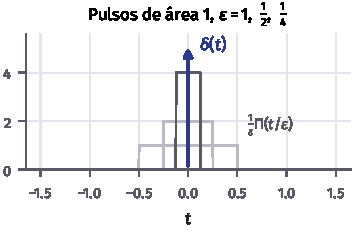
\includegraphics[width=\linewidth]{impulso_dirac}\caption{Delta de Dirac como límite de pulsos.}\end{subfigure}\hfill
  \begin{subfigure}{0.45\linewidth}\centering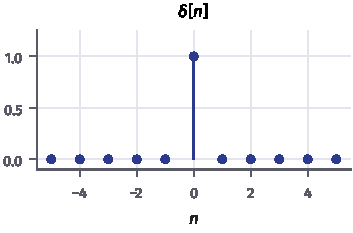
\includegraphics[width=\linewidth]{impulso_kronecker}\caption{Delta de Kronecker.}\end{subfigure}
  \caption{Impulsos continuo y discreto.}
\end{figure}

\subsection{Escalón y rampa}

\[
  u(t)=\begin{cases}1 & t>0\\0 & t<0\end{cases}\qquad
  u[n]=\begin{cases}1 & n\ge0\\0 & n<0\end{cases}\qquad
  r(t)=t\,u(t),\qquad r[n]=n\,u[n].
\]
El valor de $u(0)$ no afecta a ninguna integral; según el contexto se toma $1$ o $\tfrac12$. Las tres señales básicas se relacionan por integración y derivación (en continuo) o por acumulación y diferencia (en discreto):
\[
  u(t)=\int_{-\infty}^{t}\delta(\tau)\dd\tau,\quad \delta(t)=\dv{u(t)}{t},\qquad
  r(t)=\int_{-\infty}^{t}u(\tau)\dd\tau,\quad u(t)=\dv{r(t)}{t},
\]
\[
  u[n]=\sum_{k=-\infty}^{n}\delta[k],\quad \delta[n]=u[n]-u[n-1],\qquad
  r[n]=\sum_{k=-\infty}^{n-1}u[k],\quad u[n]=r[n+1]-r[n].
\]
Observa el desfase de una muestra en la rampa discreta: $\sum_{k\le n}u[k]=n+1$ para $n\ge0$, es decir, $r[n+1]$. Es un detalle típico del paso de continuo a discreto: la diferencia hacia atrás y la acumulación son inversas exactas, pero no reproducen todas las fórmulas continuas sin ajustar un índice.

\subsection{Pulsos rectangular y triangular}

\[
  \rect(t)=\begin{cases}1 & \abs{t}\le\frac12\\0 & \abs{t}>\frac12\end{cases}\qquad
  \tri(t)=\begin{cases}1-\abs{t} & \abs{t}\le1\\0 & \abs{t}>1\end{cases}
\]
$\rect(t/T)$ es un pulso de anchura $T$ centrado en el origen. El pulso triangular es la convolución de dos rectangulares, $\tri=\rect\conv\rect$, lo que hace muy sencilla su transformada de Fourier (\cref{sec:frecuencia}). En discreto se usa sobre todo el pulso causal de $L$ muestras, $p_L[n]=u[n]-u[n-L]$.

\begin{figure}[ht]
  \centering
  \begin{subfigure}{0.48\linewidth}\centering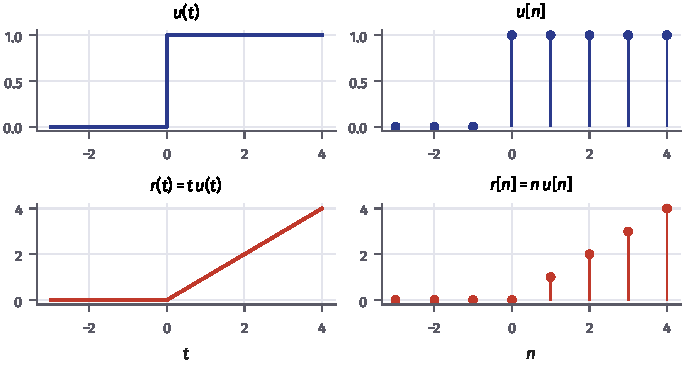
\includegraphics[width=\linewidth]{escalon_rampa}\caption{Escalón y rampa.}\end{subfigure}\hfill
  \begin{subfigure}{0.48\linewidth}\centering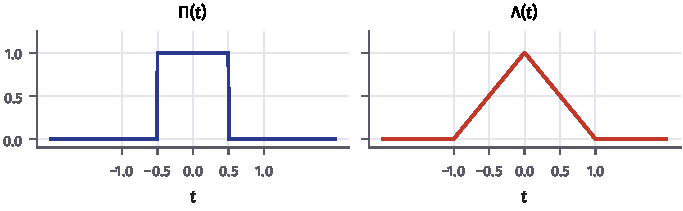
\includegraphics[width=\linewidth]{pulsos}\caption{Pulsos rectangular y triangular.}\end{subfigure}
  \caption{Señales básicas continuas y discretas.}
\end{figure}

\subsection{Exponenciales complejas continuas}

La exponencial compleja $x(t)=A\e^{j\omega_0t}$ es la señal más importante del curso. Por la fórmula de Euler,
\[
  \e^{j\theta}=\cos\theta+j\sin\theta,\qquad
  \cos\theta=\frac{\e^{j\theta}+\e^{-j\theta}}{2},\qquad
  \sin\theta=\frac{\e^{j\theta}-\e^{-j\theta}}{2j},
\]
su parte real e imaginaria son sinusoides. Es periódica para todo $\omega_0\ne0$, con $T_0=2\pi/\abs{\omega_0}$, porque $\e^{j\omega_0(t+T_0)}=\e^{j\omega_0t}\e^{\pm j2\pi}=\e^{j\omega_0t}$. Dos frecuencias distintas dan siempre señales distintas, y cuanto mayor es $\abs{\omega_0}$ más rápido oscila la señal.

La exponencial general $x(t)=C\e^{at}$, con $C=\abs{C}\e^{j\phi}$ y $a=r+j\omega_0$, es
\[
  x(t)=\abs{C}\,\e^{rt}\,\e^{j(\omega_0t+\phi)},
\]
una sinusoide compleja con envolvente exponencial decreciente ($r<0$), constante ($r=0$) o creciente ($r>0$). Si $a$ es real se reduce a la exponencial real. Estas señales son las respuestas naturales de los sistemas descritos por ecuaciones diferenciales lineales, y el exponente $a$ es un \emph{polo} del sistema (\cref{sec:lti-dc}).

\subsection{Exponenciales complejas discretas}\label{sec:exp-discreta}

La exponencial compleja discreta $x[n]=A\e^{j\Omega_0n}$ se parece a la continua, pero tiene dos diferencias fundamentales que conviene entender bien.

\begin{importante}[Primera diferencia: no siempre es periódica]
  $x[n+N]=x[n]$ exige $\e^{j\Omega_0N}=1$, es decir, $\Omega_0N=2\pi k$ para algún entero $k$. Por tanto, $\e^{j\Omega_0n}$ es periódica si y solo si
  \[
    F_0=\frac{\Omega_0}{2\pi}=\frac{k}{N}\quad\text{es racional.}
  \]
  Si la fracción $k/N$ es irreducible, el periodo fundamental es $N$.
\end{importante}

\begin{ejemplo}{Periodicidad de sinusoides discretas}{periodo-discreto}
  \begin{itemize}
    \item $\cos(\pi n/4)$: $F_0=1/8$, periodo $N=8$.
    \item $\cos(3\pi n/8)$: $F_0=3/16$, periodo $N=16$. El periodo de la sinusoide continua $\cos(3\pi t/8)$ sería $16/3$, que no es entero: la secuencia necesita $16$ muestras, tres periodos de la continua, para repetirse.
    \item $\cos(0{,}4\,n)$: $F_0=0{,}2/\pi$ es irracional y la secuencia \emph{no es periódica}, aunque $\cos(0{,}4\,t)$ sí lo sea.
  \end{itemize}
\end{ejemplo}

\begin{importante}[Segunda diferencia: frecuencias que difieren en $2\pi$ son la misma]
  \[\e^{j(\Omega_0+2\pi k)n}=\e^{j\Omega_0n}\,\e^{j2\pi kn}=\e^{j\Omega_0n}\qquad\forall k\in\Z,\]
  porque $kn$ es entero. Todas las frecuencias distintas caben en un intervalo de longitud $2\pi$, que se suele tomar $[0,2\pi)$ o $[-\pi,\pi)$.
\end{importante}

En consecuencia, la oscilación más rápida posible es la de $\Omega=\pi$, $\e^{j\pi n}=(-1)^n$, que cambia de signo en cada muestra. Las frecuencias bajas están cerca de $\Omega=0$ \emph{y también} cerca de $\Omega=2\pi$. Cuando se muestrea una sinusoide continua de frecuencia $\omega$ con periodo $T_s$, la secuencia resultante tiene $\Omega=\omega T_s$; si $\omega T_s>\pi$, la secuencia coincide con la de una frecuencia más baja. Este es el origen del \emph{aliasing}, que estudia el Tema~2.

\begin{figure}[ht]
  \centering
  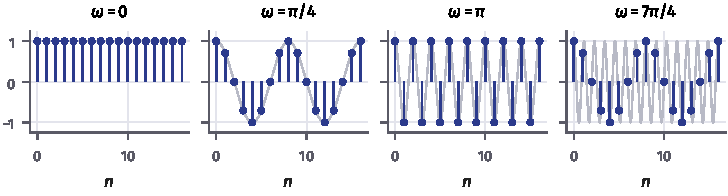
\includegraphics[width=0.8\linewidth]{coseno_discreto_frecuencias}
  \caption{$\cos(\Omega_0 n)$ para varias frecuencias: la oscilación es más rápida al acercarse a $\Omega_0=\pi$ y vuelve a ser lenta cerca de $2\pi$.}
\end{figure}

\begin{encodigo}
  Las tres secuencias son la misma aunque sus frecuencias sean $\pi/4$, $2\pi-\pi/4$ y $\pi/4+2\pi$ (la segunda, por ser un coseno, que es par):
  \codigo{alias_discreto}
\end{encodigo}

La exponencial discreta general es $x[n]=C\alpha^n$, con $C=\abs{C}\e^{j\phi}$ y $\alpha=\abs{\alpha}\e^{j\Omega_0}$:
\[
  x[n]=\abs{C}\,\abs{\alpha}^n\,\e^{j(\Omega_0n+\phi)}.
\]
Su envolvente decrece si $\abs{\alpha}<1$, es constante si $\abs{\alpha}=1$ y crece si $\abs{\alpha}>1$. Si $\alpha$ es real y negativo, la secuencia alterna de signo, algo que no tiene equivalente en la exponencial real continua. Son las respuestas naturales de las ecuaciones en diferencias, y $\alpha$ es un polo en el plano $z$.

\subsection{Otras señales: Sa, sinc, signo y chirp}

\[
  \Sa(t)=\frac{\sin t}{t},\qquad \sinc(t)=\frac{\sin(\pi t)}{\pi t},\qquad
  \sgn(t)=\begin{cases}1 & t>0\\0 & t=0\\-1 & t<0\end{cases}
\]
con $\Sa(0)=\sinc(0)=1$, de modo que $\sinc(t)=\Sa(\pi t)$. La función $\sinc$ se anula en todos los enteros no nulos; es la transformada de Fourier del pulso rectangular y el interpolador ideal del Tema~2. Tanto \texttt{np.sinc} como \texttt{sinc} de Matlab calculan $\sin(\pi t)/(\pi t)$.

Las ondas cuadrada y triangular son periódicas y solo contienen armónicos impares (\cref{sec:frecuencia}). El \emph{chirp} lineal, $x(t)=\cos\big(2\pi(f_0t+\tfrac\beta2t^2)\big)$, tiene una frecuencia instantánea $f_i(t)=\frac{1}{2\pi}\dv{\theta}{t}=f_0+\beta t$ que crece linealmente; se usa en radar, sonar y para medir respuestas en frecuencia.

\begin{encodigo}
  Para representar secuencias basta un vector de índices y comparaciones lógicas:
  \codigo{senales_basicas}
\end{encodigo}

\begin{flushright}\small\color{pdsgris}Ejercicios 1, 2 y 9. \herramienta{T1-exponencial-continua, T1-exponencial-discreta, T1-continua-discreta}.\end{flushright}

% =====================================================================
\section{Operaciones con señales}\label{sec:operaciones}

\subsection{Transformaciones de la variable independiente}

Estas operaciones cambian el eje de tiempos sin alterar los valores que toma la señal: $y(t)=x\big(f(t)\big)$. Cuando $f$ es afín se reducen a tres operaciones básicas.

\begin{itemize}
  \item \textbf{Desplazamiento}: $y(t)=x(t-t_0)$. Si $t_0>0$ es un \emph{retardo}: la señal se desplaza hacia la derecha, porque $y$ toma en $t=t_0$ el valor que $x$ tenía en $t=0$. Si $t_0<0$ es un \emph{adelanto}. En discreto, $y[n]=x[n-n_0]$ con $n_0$ entero.
  \item \textbf{Inversión}: $y(t)=x(-t)$, reflejo respecto al origen.
  \item \textbf{Escalado}: $y(t)=x(\alpha t)$ con $\alpha>0$ comprime la señal si $\alpha>1$ y la expande si $\alpha<1$. Es reversible: $x(t)=y(t/\alpha)$.
\end{itemize}

\begin{figure}[ht]
  \centering
  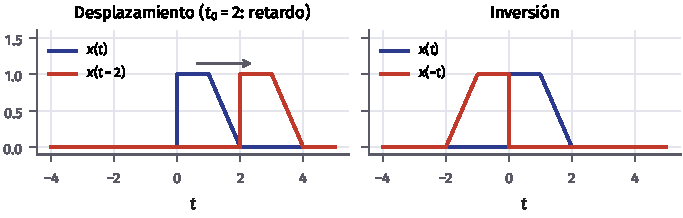
\includegraphics[width=0.62\linewidth]{desplazamiento_inversion}
  \caption{Desplazamiento e inversión de una señal continua.}
\end{figure}

En discreto el escalado no es reversible en general, porque el índice tiene que seguir siendo entero. El \emph{diezmado} $y[n]=x[Mn]$, con $M$ entero positivo, se queda con una de cada $M$ muestras y descarta las demás: se pierde información. La \emph{expansión} por un factor $L$ define $y[n]=x[n/L]$ cuando $n$ es múltiplo de $L$ y $y[n]=0$ en otro caso; las muestras intermedias se rellenan después mediante interpolación (Tema~2).

\begin{figure}[ht]
  \centering
  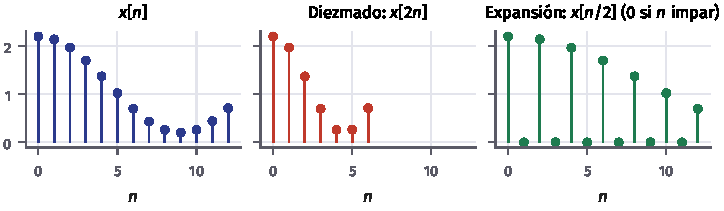
\includegraphics[width=0.7\linewidth]{diezmado_interpolacion}
  \caption{Diezmado por $M=2$ y expansión por $L=2$ de una secuencia.}
\end{figure}

\paragraph{Transformaciones combinadas.} Para dibujar $y(t)=x(\alpha t+\beta)$ hay un procedimiento que no falla: primero desplazar, $v(t)=x(t+\beta)$, y después escalar (e invertir si $\alpha<0$), $y(t)=v(\alpha t)=x(\alpha t+\beta)$. Si se escala primero, el desplazamiento que hay que aplicar después es $\beta/\alpha$, porque $x(\alpha t+\beta)=x\big(\alpha(t+\beta/\alpha)\big)$. Una comprobación rápida consiste en seguir un punto: el valor que $x$ tenía en $t=0$ aparece en $y$ cuando $\alpha t+\beta=0$.

\begin{ejemplo}{$y(t)=x(2t+1)$}{combinada}
  Primero $v(t)=x(t+1)$, que adelanta $x$ una unidad; después $y(t)=v(2t)$, que comprime $v$ a la mitad. El punto $t=0$ de $x$ aparece en $y$ en $2t+1=0$, es decir, en $t=-\tfrac12$. Si $x$ es no nula en $[-1,1]$, $y$ es no nula en $[-1,0]$.
  \begin{center}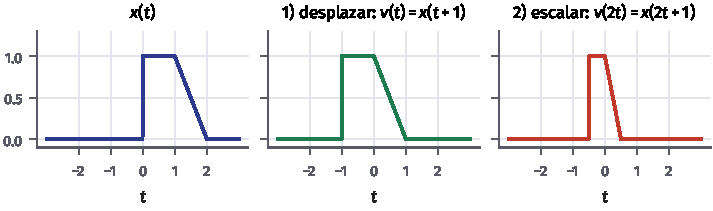
\includegraphics[width=0.75\linewidth]{transformacion_combinada}\end{center}
\end{ejemplo}

\subsection{Operaciones sobre la amplitud}

Las operaciones punto a punto se aplican igual a señales continuas y discretas: suma, producto (que aparece en la modulación y el enventanado), escalado de amplitud y cociente (donde el denominador no se anule). Además, para señales continuas se definen la derivada y la integral acumulada, y para secuencias sus análogos discretos:
\[
  \text{diferencia: } y[n]=x[n]-x[n-1],\qquad \text{acumulación: } y[n]=\sum_{k=-\infty}^{n}x[k].
\]
La diferencia es la versión discreta de la derivada y la acumulación, la de la integral: por ejemplo $u[n]-u[n-1]=\delta[n]$ y $\sum_{k\le n}\delta[k]=u[n]$, igual que $u'(t)=\delta(t)$.

\begin{nota}[Producto y convolución]
  El producto $x_1(t)\,x_2(t)$ y la convolución $(x_1\conv x_2)(t)$ son operaciones muy distintas. En estos apuntes el producto se escribe por yuxtaposición o con un punto, y el asterisco $\conv$ se reserva siempre para la convolución.
\end{nota}

\begin{flushright}\small\color{pdsgris}\herramienta{T1-variable-independiente}.\end{flushright}

% =====================================================================
\section{Convolución}\label{sec:convolucion}

\begin{definicion}{Convolución}{convolucion}
  \[
    (x\conv h)(t)=\int_{-\infty}^{\infty}x(\tau)\,h(t-\tau)\dd\tau,\qquad
    (x\conv h)[n]=\sum_{k=-\infty}^{\infty}x[k]\,h[n-k].
  \]
\end{definicion}

La convolución es la operación central de los sistemas LTI: en la \cref{sec:lti} veremos que la salida de cualquier sistema LTI es la convolución de la entrada con su respuesta al impulso. Para calcularla a mano conviene seguir el procedimiento gráfico, para cada valor de $t$:
\begin{enumerate}
  \item reflejar $h(\tau)$ para obtener $h(-\tau)$;
  \item desplazarla hasta $h(t-\tau)$;
  \item multiplicar por $x(\tau)$;
  \item integrar (o sumar) el producto en $\tau$.
\end{enumerate}
A medida que $t$ avanza, la versión reflejada de $h$ se desliza sobre $x$ y conviene dividir el eje $t$ en intervalos según cómo se solapen las dos señales.

\begin{propiedad}{Convolución}{conv}
  \begin{itemize}
    \item Conmutativa: $x\conv h=h\conv x$.
    \item Asociativa: $(x\conv h_1)\conv h_2=x\conv(h_1\conv h_2)$.
    \item Distributiva respecto a la suma: $x\conv(h_1+h_2)=x\conv h_1+x\conv h_2$.
    \item Elemento neutro y desplazamiento: $x\conv\delta=x$, \ $x(t)\conv\delta(t-t_0)=x(t-t_0)$.
    \item Con el escalón: $(x\conv u)(t)=\int_{-\infty}^{t}x(\tau)\dd\tau$, \ $(x\conv u)[n]=\sum_{k\le n}x[k]$.
    \item Duración: si $x$ es no nula en $[a,b]$ y $h$ en $[c,d]$, $x\conv h$ es no nula como mucho en $[a+c,\,b+d]$.
  \end{itemize}
\end{propiedad}

\begin{ejemplo}{Convolución continua de un pulso y una exponencial}{conv-cont}
  Sean $x(t)=u(t)-u(t-1)$ y $h(t)=\e^{-t}u(t)$. Usamos $y(t)=\int x(\tau)\,h(t-\tau)\dd\tau$, con $x(\tau)=1$ en $[0,1]$ y $h(t-\tau)=\e^{-(t-\tau)}$ para $\tau\le t$.
  \begin{itemize}
    \item Si $t<0$, las señales no se solapan y $y(t)=0$.
    \item Si $0\le t\le1$, el solape es $[0,t]$: $y(t)=\int_0^t\e^{-(t-\tau)}\dd\tau=\e^{-t}(\e^{t}-1)=1-\e^{-t}$.
    \item Si $t>1$, el pulso queda entero dentro: $y(t)=\int_0^1\e^{-(t-\tau)}\dd\tau=(\e-1)\,\e^{-t}$.
  \end{itemize}
  La salida es continua en $t=1$, donde ambas expresiones valen $1-\e^{-1}\approx0{,}632$.
  \begin{center}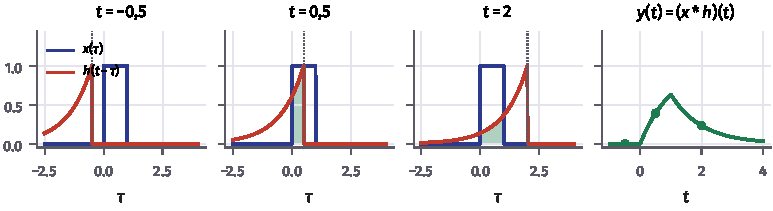
\includegraphics[width=0.85\linewidth]{convolucion_pasos}\end{center}
\end{ejemplo}

\begin{ejemplo}{Convolución discreta}{conv-disc}
  Sean $x[n]=\{\underline{1},2,1\}$ y $h[n]=\{\underline{1},1,1,1\}$, donde el subrayado marca $n=0$. Por la descomposición en impulsos, $x\conv h=x[0]h[n]+x[1]h[n-1]+x[2]h[n-2]$, y basta sumar copias desplazadas de $h$:
  \begin{center}
  \begin{tabular}{@{}c|cccccc@{}}
    $n$ & 0 & 1 & 2 & 3 & 4 & 5\\\hline
    $x[0]h[n]$ & 1 & 1 & 1 & 1 & & \\
    $x[1]h[n-1]$ & & 2 & 2 & 2 & 2 & \\
    $x[2]h[n-2]$ & & & 1 & 1 & 1 & 1\\\hline
    $y[n]$ & 1 & 3 & 4 & 4 & 3 & 1
  \end{tabular}
  \end{center}
  Si $x$ tiene $N_x$ muestras y $h$ tiene $N_h$, la convolución tiene $N_x+N_h-1$; si empiezan en $n_x$ y $n_h$, el resultado empieza en $n_x+n_h$.
\end{ejemplo}

\begin{encodigo}
  \texttt{np.convolve} y \texttt{conv} trabajan con vectores sin índice: el índice inicial del resultado hay que llevarlo aparte (es la suma de los índices iniciales).
  \codigo{convolucion}
\end{encodigo}

\begin{flushright}\small\color{pdsgris}Ejercicios 5 y 6. \herramienta{T1-convolucion-continua, T1-convolucion-discreta}.\end{flushright}

% =====================================================================
\section{Representación en frecuencia}\label{sec:frecuencia}

\subsection{La idea: descomponer en exponenciales complejas}

Las exponenciales complejas $\e^{j\omega t}$ y $\e^{j\Omega n}$ son \emph{autofunciones} de los sistemas LTI: atraviesan el sistema sin cambiar de forma, solo multiplicadas por un número complejo (\cref{sec:autofunciones}). Si una señal se escribe como suma o integral de exponenciales complejas, la respuesta del sistema se obtiene sumando las respuestas a cada una. Según la señal sea continua o discreta, periódica o aperiódica, se usa una de cuatro representaciones:

\begin{center}
  \renewcommand{\arraystretch}{1.2}
  \begin{tabular}{@{}lll@{}}
    \toprule
    & Tiempo continuo & Tiempo discreto\\\midrule
    Periódica & Serie de Fourier: $c_k$ & Serie de Fourier discreta (DFS): $c_k$\\
    Aperiódica & Transformada de Fourier (CTFT): $\Xc$ & Transformada de Fourier (DTFT): $\Xd$\\\bottomrule
  \end{tabular}
\end{center}

Hay una dualidad que conviene retener: la periodicidad en un dominio se corresponde con un espectro discreto (de líneas) en el otro, y el tiempo discreto se corresponde con un espectro periódico.

\subsection{Serie de Fourier de señales continuas periódicas}

Sea $x(t)$ periódica de periodo $T_0$ y frecuencia fundamental $\omega_0=2\pi/T_0$. Su serie de Fourier exponencial es
\[
  x(t)=\sum_{k=-\infty}^{\infty}c_k\,\e^{jk\omega_0t},\qquad
  c_k=\frac{1}{T_0}\int_{T_0}x(t)\,\e^{-jk\omega_0t}\dd t.
\]
La fórmula de análisis se obtiene multiplicando la de síntesis por $\e^{-jm\omega_0t}$ e integrando en un periodo: todas las exponenciales con $k\ne m$ integran cero (son ortogonales) y solo queda $T_0c_m$. El coeficiente $c_0$ es el valor medio de la señal y los pares $\abs{c_k}$, $\arg c_k$ forman su espectro de líneas.

Si $x$ es real, $c_{-k}=c_k^*$ y la serie se puede escribir en forma trigonométrica:
\[
  x(t)=\frac{a_0}{2}+\sum_{k=1}^{\infty}\big(a_k\cos(k\omega_0t)+b_k\sin(k\omega_0t)\big),
\]
\[
  a_k=\frac{2}{T_0}\int_{T_0}x(t)\cos(k\omega_0t)\dd t,\quad
  b_k=\frac{2}{T_0}\int_{T_0}x(t)\sin(k\omega_0t)\dd t,
\]
con $c_k=\tfrac12(a_k-jb_k)$. Si $x$ es par, todos los $b_k$ se anulan; si es impar, se anulan los $a_k$.

\begin{propiedad}{Parseval para series de Fourier}{parseval-sf}
  \[
    P_x=\frac{1}{T_0}\int_{T_0}\abs{x(t)}^2\dd t=\sum_{k=-\infty}^{\infty}\abs{c_k}^2.
  \]
  La potencia de la señal es la suma de las potencias de sus armónicos.
\end{propiedad}

\begin{ejemplo}{Onda cuadrada}{cuadrada}
  Sea la onda cuadrada par de amplitud $\pm1$ y ciclo de trabajo del 50\,\%: $x(t)=1$ para $\abs{t}<T_0/4$ y $x(t)=-1$ para $T_0/4<\abs{t}<T_0/2$. Su valor medio es $c_0=0$. Escribiendo $x=2p-1$, donde $p$ es un tren de pulsos de altura $1$ y anchura $T_0/2$, para $k\ne0$:
  \[
    c_k=\frac{2}{T_0}\int_{-T_0/4}^{T_0/4}\e^{-jk\omega_0t}\dd t
    =\frac{2}{T_0}\cdot\frac{2\sin(k\omega_0T_0/4)}{k\omega_0}
    =\frac{\sin(\pi k/2)}{\pi k/2}=\sinc(k/2).
  \]
  Los coeficientes pares son nulos y los impares valen $\pm2/(\pi k)$, de modo que
  \[
    x(t)=\frac{4}{\pi}\Big(\cos\omega_0t-\tfrac13\cos3\omega_0t+\tfrac15\cos5\omega_0t-\cdots\Big).
  \]
  Comprobación con Parseval: $P_x=1$ y $\sum_k\abs{c_k}^2=2\sum_{k\text{ impar}}\frac{4}{\pi^2k^2}=\frac{8}{\pi^2}\cdot\frac{\pi^2}{8}=1$.
  \begin{center}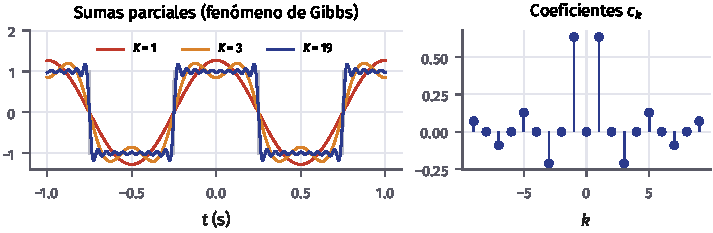
\includegraphics[width=0.72\linewidth]{serie_fourier_cuadrada}\end{center}
  Cerca de las discontinuidades, las sumas parciales sobrepasan el salto en torno a un 9\,\% por mucho que crezca el número de armónicos: es el \emph{fenómeno de Gibbs}. El pico se estrecha, pero su altura no disminuye.
\end{ejemplo}

\begin{encodigo}
  Suma parcial de la serie de la onda cuadrada con $K$ armónicos. Prueba con $K=1,3,19,99$.
  \codigo{serie_fourier}
\end{encodigo}

\subsection{Serie de Fourier discreta}

Si $x[n]$ es periódica de periodo $N$, solo hay $N$ exponenciales $\e^{j\frac{2\pi}{N}kn}$ distintas (por la segunda diferencia de la \cref{sec:exp-discreta}), de modo que la serie es una suma finita:
\[
  x[n]=\sum_{k=0}^{N-1}c_k\,\e^{j\frac{2\pi}{N}kn},\qquad
  c_k=\frac{1}{N}\sum_{n=0}^{N-1}x[n]\,\e^{-j\frac{2\pi}{N}kn},\qquad c_{k+N}=c_k.
\]
No hay problemas de convergencia ni fenómeno de Gibbs: son $N$ ecuaciones con $N$ incógnitas. Para $x$ real, la forma trigonométrica es
\[
  x[n]=\frac{a_0}{2}+\sum_{k=1}^{L}\Big(a_k\cos\big(\tfrac{2\pi}{N}kn\big)+b_k\sin\big(\tfrac{2\pi}{N}kn\big)\Big)\;\Big[+\tfrac{a_{N/2}}{2}(-1)^n\Big],
\]
con $a_k=\frac2N\sum_{n=0}^{N-1}x[n]\cos\big(\tfrac{2\pi}{N}kn\big)$, $b_k=\frac2N\sum_{n=0}^{N-1}x[n]\sin\big(\tfrac{2\pi}{N}kn\big)$ y $L=(N-1)/2$ si $N$ es impar. Si $N$ es par, $L=N/2-1$ y hay que añadir el término entre corchetes, que corresponde a la frecuencia $\Omega=\pi$. La DFT de un periodo, que estudia el Tema~3, es $X[k]=Nc_k$.

\subsection{Transformada de Fourier en tiempo continuo}

Cuando el periodo $T_0$ de una señal crece sin límite, las líneas del espectro se acercan ($\omega_0\to0$) y la serie se convierte en una integral. Así se obtiene la transformada de Fourier:
\[
  \Xc=\int_{-\infty}^{\infty}x(t)\,\e^{-j\omega t}\dd t,\qquad
  x(t)=\frac{1}{2\pi}\int_{-\infty}^{\infty}\Xc\,\e^{j\omega t}\dd\omega.
\]
Existe si $x$ es absolutamente integrable, $\int\abs{x}\dd t<\infty$; admitiendo deltas en frecuencia, se extiende a señales de potencia como las sinusoides o el escalón. Si $x$ es real, $X(-j\omega)=X^*(j\omega)$.

\begin{ejemplo}{Dos transformadas básicas}{ctft}
  \begin{itemize}
    \item $x(t)=\e^{-at}u(t)$, $a>0$: \ $\Xc=\int_0^\infty\e^{-(a+j\omega)t}\dd t=\dfrac{1}{a+j\omega}$. El módulo, $1/\sqrt{a^2+\omega^2}$, es máximo en $\omega=0$ y decae: es una señal «de baja frecuencia».
    \item $x(t)=\rect(t/T)$: \ $\Xc=\int_{-T/2}^{T/2}\e^{-j\omega t}\dd t=\dfrac{2\sin(\omega T/2)}{\omega}=T\sinc\Big(\dfrac{\omega T}{2\pi}\Big)$. Los ceros están en $\omega=2\pi k/T$: cuanto más corto es el pulso, más ancho es su espectro.
  \end{itemize}
  \begin{center}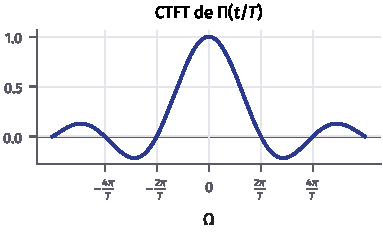
\includegraphics[width=0.5\linewidth]{espectro_ctft_pulso}\end{center}
\end{ejemplo}

\begin{center}
  \renewcommand{\arraystretch}{1.3}
  \begin{tabular}{@{}ll@{\qquad}ll@{}}
    \toprule
    $x(t)$ & $\Xc$ & $x(t)$ & $\Xc$\\\midrule
    $\delta(t)$ & $1$ & $\e^{-at}u(t)$, $a>0$ & $\dfrac{1}{a+j\omega}$\\
    $1$ & $2\pi\,\delta(\omega)$ & $\rect(t/T)$ & $T\sinc\!\big(\tfrac{\omega T}{2\pi}\big)$\\
    $\e^{j\omega_0t}$ & $2\pi\,\delta(\omega-\omega_0)$ & $\tri(t)$ & $\sinc^2\!\big(\tfrac{\omega}{2\pi}\big)$\\
    $\cos(\omega_0t)$ & $\pi[\delta(\omega-\omega_0)+\delta(\omega+\omega_0)]$ & $\sgn(t)$ & $\dfrac{2}{j\omega}$\\\bottomrule
  \end{tabular}
\end{center}

\subsection{Transformada de Fourier en tiempo discreto}

\[
  \Xd=\sum_{n=-\infty}^{\infty}x[n]\,\e^{-j\Omega n},\qquad
  x[n]=\frac{1}{2\pi}\int_{2\pi}\Xd\,\e^{j\Omega n}\dd\Omega.
\]
La DTFT existe si $\sum\abs{x[n]}<\infty$. Su propiedad más característica es que es \emph{periódica en $\Omega$ con periodo $2\pi$}, consecuencia directa de que $\e^{-j(\Omega+2\pi)n}=\e^{-j\Omega n}$. Basta, por tanto, representarla en $[-\pi,\pi)$ o en $[0,2\pi)$. Numéricamente se evalúa con \texttt{freqz}.

\begin{ejemplo}{Exponencial causal y pulso}{dtft}
  \begin{itemize}
    \item $x[n]=a^nu[n]$, $\abs{a}<1$: \ $\Xd=\sum_{n\ge0}(a\e^{-j\Omega})^n=\dfrac{1}{1-a\e^{-j\Omega}}$.
    \item $x[n]=u[n]-u[n-L]$: suma geométrica finita,
    \[
      \Xd=\sum_{n=0}^{L-1}\e^{-j\Omega n}=\frac{1-\e^{-j\Omega L}}{1-\e^{-j\Omega}}
      =\e^{-j\Omega\frac{L-1}{2}}\,\frac{\sin(\Omega L/2)}{\sin(\Omega/2)}.
    \]
    Es el equivalente discreto del $\sinc$: el cociente de senos se llama a veces \emph{núcleo de Dirichlet}. Sus ceros están en $\Omega=2\pi k/L$, $k\ne0,L,2L,\ldots$
  \end{itemize}
  \begin{center}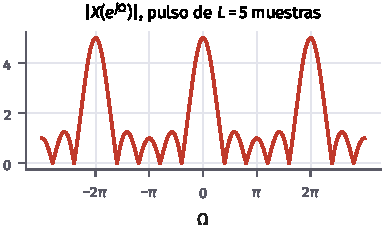
\includegraphics[width=0.5\linewidth]{espectro_dtft_pulso}\end{center}
\end{ejemplo}

\begin{encodigo}
  \texttt{freqz} evalúa $\sum_n x[n]\e^{-j\Omega n}$ en una rejilla de frecuencias; con la opción \texttt{whole} cubre $[0,2\pi)$ y deja ver la periodicidad.
  \codigo{dtft_pulso}
\end{encodigo}

\subsection{Propiedades de la transformada de Fourier}

\begin{center}
  \small
  \renewcommand{\arraystretch}{1.35}
  \begin{tabular}{@{}lll@{}}
    \toprule
    Propiedad & CTFT & DTFT\\\midrule
    Linealidad & $a x_1+b x_2\parF aX_1+bX_2$ & ídem\\
    Desplazamiento & $x(t-t_0)\parF\e^{-j\omega t_0}\Xc$ & $x[n-n_0]\parF\e^{-j\Omega n_0}\Xd$\\
    Modulación & $\e^{j\omega_0t}x(t)\parF X(j(\omega-\omega_0))$ & $\e^{j\Omega_0n}x[n]\parF X(\e^{j(\Omega-\Omega_0)})$\\
    Escalado & $x(at)\parF\frac{1}{\abs{a}}X\big(j\tfrac{\omega}{a}\big)$ & —\\
    Derivada / diferencia & $\dv{x}{t}\parF j\omega\,\Xc$ & $x[n]-x[n-1]\parF(1-\e^{-j\Omega})\Xd$\\
    Convolución & $x\conv h\parF\Xc H(j\omega)$ & $x\conv h\parF\Xd H(\e^{j\Omega})$\\
    Producto & $x\,y\parF\frac{1}{2\pi}(X\conv Y)(j\omega)$ & $x\,y\parF\frac{1}{2\pi}\int_{2\pi}X(\e^{j\theta})Y(\e^{j(\Omega-\theta)})\dd\theta$\\
    Parseval & $\int\abs{x}^2\dd t=\frac{1}{2\pi}\int\abs{X}^2\dd\omega$ & $\sum\abs{x}^2=\frac{1}{2\pi}\int_{2\pi}\abs{X}^2\dd\Omega$\\\bottomrule
  \end{tabular}
\end{center}

Tres de ellas merecen un comentario. La propiedad de \emph{desplazamiento} dice que retrasar una señal no cambia el módulo de su espectro, solo añade una fase lineal en la frecuencia. La de \emph{modulación} dice que multiplicar por una exponencial desplaza el espectro: es la base de la modulación en comunicaciones. Y la de \emph{convolución} es la clave del curso: \emph{filtrar es multiplicar espectros}. Un sistema LTI con respuesta en frecuencia $H$ deja pasar las frecuencias donde $\abs{H}$ es grande y atenúa aquellas donde es pequeño.

La DTFT no tiene propiedad de escalado: diezmar o expandir una secuencia cambia su espectro de una forma más complicada, que se estudia en el Tema~2 al hablar de cambio de frecuencia de muestreo.

\subsection{Transformada de Laplace}

La transformada de Fourier no existe para señales que crecen, como $\e^{t}u(t)$, ni es la herramienta más cómoda para resolver ecuaciones diferenciales. La transformada de Laplace la generaliza sustituyendo $j\omega$ por una variable compleja $s=\sigma+j\omega$:
\[
  X(s)=\Lap\{x(t)\}=\int_{-\infty}^{\infty}x(t)\,\e^{-st}\dd t.
\]
Equivale a la transformada de Fourier de $x(t)\e^{-\sigma t}$: el factor $\e^{-\sigma t}$ hace converger la integral para algunos valores de $\sigma$. El conjunto de valores de $s$ en que converge es la \emph{región de convergencia} (ROC), que es siempre una franja vertical $\sigma_1<\Re\{s\}<\sigma_2$ y que no contiene polos.

\begin{importante}[La ROC es parte de la transformada]
  \[
    \e^{-at}u(t)\parL\frac{1}{s+a},\ \ \Re\{s\}>-a,\qquad
    -\e^{-at}u(-t)\parL\frac{1}{s+a},\ \ \Re\{s\}<-a.
  \]
  La misma expresión algebraica corresponde a dos señales distintas, una causal y otra anticausal. Sin la ROC, la transformada no determina la señal.
\end{importante}

Para la primera, $\int_0^\infty\e^{-(s+a)t}\dd t$ converge solo si $\Re\{s+a\}>0$. Para la segunda, $-\int_{-\infty}^0\e^{-(s+a)t}\dd t$ converge solo si $\Re\{s+a\}<0$. En general, una señal causal tiene la ROC a la derecha de su polo más a la derecha, una anticausal a la izquierda del polo más a la izquierda, y una bilateral, en una franja entre polos.

Si la ROC contiene el eje imaginario, la transformada de Fourier existe y se obtiene evaluando en él: $\Xc=X(s)|_{s=j\omega}$. La versión \emph{unilateral}, $\int_{0^-}^\infty$, coincide con la bilateral para señales causales y tiene la ventaja de incorporar las condiciones iniciales en la propiedad de la derivada, por lo que es la que se usa para resolver ecuaciones diferenciales con condiciones iniciales no nulas.

\begin{center}
  \small
  \renewcommand{\arraystretch}{1.3}
  \begin{tabular}{@{}lll@{\qquad}ll@{}}
    \toprule
    $x(t)$ & $X(s)$ & ROC & Propiedad & \\\midrule
    $\delta(t)$ & $1$ & todo $\C$ & Linealidad & $a x_1+b x_2\parL aX_1+bX_2$\\
    $u(t)$ & $1/s$ & $\Re\{s\}>0$ & Desplazamiento & $x(t-t_0)\parL\e^{-st_0}X(s)$\\
    $t\,u(t)$ & $1/s^2$ & $\Re\{s\}>0$ & Desplaz. en $s$ & $\e^{s_0t}x(t)\parL X(s-s_0)$\\
    $\e^{-at}u(t)$ & $\dfrac{1}{s+a}$ & $\Re\{s\}>-a$ & Derivada & $\dv{x}{t}\parL sX(s)$\\
    $\cos(\omega_0t)u(t)$ & $\dfrac{s}{s^2+\omega_0^2}$ & $\Re\{s\}>0$ & \quad (unilateral) & $\dv{x}{t}\parL sX(s)-x(0^-)$\\
    $\sin(\omega_0t)u(t)$ & $\dfrac{\omega_0}{s^2+\omega_0^2}$ & $\Re\{s\}>0$ & Integral & $\int_{-\infty}^{t}x\dd\tau\parL X(s)/s$\\
    $\e^{-at}\cos(\omega_0t)u(t)$ & $\dfrac{s+a}{(s+a)^2+\omega_0^2}$ & $\Re\{s\}>-a$ & Convolución & $x\conv h\parL X(s)H(s)$\\\bottomrule
  \end{tabular}
\end{center}

\subsection{Transformada Z}

La transformada Z es el equivalente discreto de la de Laplace:
\[
  X(z)=\Zt\{x[n]\}=\sum_{n=-\infty}^{\infty}x[n]\,z^{-n},\qquad z=r\e^{j\Omega}\in\C.
\]
Con $z=r\e^{j\Omega}$ es la DTFT de $x[n]r^{-n}$. Su ROC es una corona $r_1<\abs{z}<r_2$ que no contiene polos. Igual que en Laplace, la ROC forma parte de la transformada:
\[
  a^nu[n]\parZ\frac{1}{1-az^{-1}},\ \ \abs{z}>\abs{a},\qquad
  -a^nu[-n-1]\parZ\frac{1}{1-az^{-1}},\ \ \abs{z}<\abs{a}.
\]
Una secuencia causal tiene la ROC fuera de un círculo, $\abs{z}>\max\abs{p_i}$; una anticausal, dentro de un círculo; y una bilateral, en una corona entre polos.

\begin{ejemplo}{Una secuencia bilateral}{z-bilateral}
  $x[n]=(0{,}5)^nu[n]-2^nu[-n-1]$. Cada término aporta su transformada con su ROC: $\abs{z}>0{,}5$ para el primero y $\abs{z}<2$ para el segundo. La ROC de la suma es la intersección, $0{,}5<\abs{z}<2$, y
  \[
    X(z)=\frac{1}{1-0{,}5z^{-1}}+\frac{1}{1-2z^{-1}}.
  \]
  Como la ROC contiene la circunferencia unidad, la DTFT existe y vale $X(\e^{j\Omega})$. Si el segundo término fuera $3^nu[n]$, las ROC ($\abs{z}>0{,}5$ y $\abs{z}>3$) también se cortarían, pero la circunferencia unidad quedaría fuera y la DTFT no existiría.
\end{ejemplo}

Si la ROC contiene la circunferencia unidad, la DTFT existe y $\Xd=X(z)|_{z=\e^{j\Omega}}$. La versión unilateral, $\sum_{n\ge0}$, incorpora las condiciones iniciales a la propiedad de desplazamiento.

\begin{center}
  \small
  \renewcommand{\arraystretch}{1.3}
  \begin{tabular}{@{}lll@{\qquad}ll@{}}
    \toprule
    $x[n]$ & $X(z)$ & ROC & Propiedad & \\\midrule
    $\delta[n]$ & $1$ & todo $\C$ & Linealidad & $a x_1+b x_2\parZ aX_1+bX_2$\\
    $u[n]$ & $\dfrac{1}{1-z^{-1}}$ & $\abs{z}>1$ & Desplazamiento & $x[n-n_0]\parZ z^{-n_0}X(z)$\\
    $a^nu[n]$ & $\dfrac{1}{1-az^{-1}}$ & $\abs{z}>\abs{a}$ & \quad (unilateral) & $x[n-1]\parZ z^{-1}X(z)+x[-1]$\\
    $n\,a^nu[n]$ & $\dfrac{az^{-1}}{(1-az^{-1})^2}$ & $\abs{z}>\abs{a}$ & \quad (unilateral) & $x[n+1]\parZ zX(z)-z\,x[0]$\\
    $\cos(\Omega_0n)u[n]$ & $\dfrac{1-\cos\Omega_0\,z^{-1}}{1-2\cos\Omega_0\,z^{-1}+z^{-2}}$ & $\abs{z}>1$ & Escalado en $z$ & $a^nx[n]\parZ X(z/a)$\\
    $\sin(\Omega_0n)u[n]$ & $\dfrac{\sin\Omega_0\,z^{-1}}{1-2\cos\Omega_0\,z^{-1}+z^{-2}}$ & $\abs{z}>1$ & Convolución & $x\conv h\parZ X(z)H(z)$\\\bottomrule
  \end{tabular}
\end{center}

\subsection{Relación entre las transformadas}

\begin{figure}[ht]
  \centering
  \begin{tikzpicture}[node distance=1.1cm and 4.2cm, every node/.style={font=\small}]
    \node[bloque] (L) {Laplace $X(s)$};
    \node[bloque, right=of L] (Z) {Z \ $X(z)$};
    \node[bloque, below=of L] (F) {CTFT $\Xc$};
    \node[bloque, below=of Z] (D) {DTFT $\Xd$};
    \draw[flecha] (L) -- node[left, align=right]{$s=j\omega$\\\scriptsize(ROC $\ni$ eje $j\omega$)} (F);
    \draw[flecha] (Z) -- node[right, align=left]{$z=\e^{j\Omega}$\\\scriptsize(ROC $\ni$ $\abs{z}=1$)} (D);
    \draw[flecha, dashed] (L) -- node[above]{muestreo $t=nT_s$} node[below]{$z=\e^{sT_s}$} (Z);
    \draw[flecha, dashed] (F) -- node[below]{$\Omega=\omega T_s$} (D);
  \end{tikzpicture}
  \caption{Relación entre las transformadas continuas y discretas.}
\end{figure}

Laplace y Z se usan para resolver ecuaciones diferenciales y en diferencias y para estudiar la función de transferencia, los polos, los ceros y la estabilidad de los sistemas LTI. Fourier se usa para describir el contenido en frecuencia de las señales y la respuesta en frecuencia de los sistemas estables. La relación $z=\e^{sT_s}$ entre los planos $s$ y $z$, que aparece al muestrear, transforma el semiplano izquierdo en el interior de la circunferencia unidad y el eje $j\omega$ en la propia circunferencia; se estudia en el Tema~2 y se usa en el diseño de filtros IIR.

\begin{flushright}\small\color{pdsgris}Ejercicios 7 y 8. \herramienta{T1-serie-fourier, T1-propiedades-fourier, T1-region-convergencia}.\end{flushright}

% =====================================================================
\section{Propiedades de los sistemas}\label{sec:propiedades}

\subsection{Clasificación general}

Según el número de entradas y salidas, un sistema es SISO (una entrada y una salida), MIMO (varias de cada) o de alguno de los tipos intermedios SIMO y MISO. Un sistema sin entradas que evoluciona desde sus condiciones iniciales es \emph{autónomo}. Según el tipo de señal, es continuo, discreto o híbrido (los conversores A/D y D/A). Y es determinista o estocástico según intervengan o no procesos aleatorios en la relación entre la entrada y la salida.

\subsection{Memoria, causalidad, estabilidad e invertibilidad}

\begin{definicion}{Memoria}{memoria}
  Un sistema es \emph{sin memoria} (estático) si la salida en cada instante depende solo de la entrada en ese mismo instante. En otro caso es \emph{con memoria} (dinámico).
\end{definicion}

Una resistencia, $v(t)=R\,i(t)$, o el sistema $y[n]=x^2[n]$ no tienen memoria. Un condensador, $v(t)=\frac1C\int_{-\infty}^{t}i(\tau)\dd\tau$, o el sistema $y[n]=x[n]+x[n-1]$ sí la tienen. Los sistemas continuos con memoria se describen con ecuaciones diferenciales y los discretos, con ecuaciones en diferencias.

\begin{definicion}{Causalidad}{causal}
  Un sistema es \emph{causal} si la salida en cada instante $t_0$ solo depende de la entrada en instantes $t\le t_0$.
\end{definicion}

Un sistema no causal usa valores futuros de la entrada y no se puede implementar en tiempo real, pero sí sobre datos grabados: el procesado de audio en posproducción o el de imágenes, donde la variable no es el tiempo, usan a menudo sistemas no causales. La media $y[n]=\frac13(x[n]+x[n-1]+x[n-2])$ es causal; la media centrada $y[n]=\frac13(x[n+1]+x[n]+x[n-1])$ no lo es, aunque basta retrasar la salida una muestra para hacerla causal. Ese retardo es el precio de «usar el futuro».

\begin{definicion}{Estabilidad BIBO}{bibo}
  Un sistema es estable en sentido BIBO (\emph{bounded input, bounded output}) si toda entrada acotada produce una salida acotada: $\abs{x}\le B_x<\infty$ implica $\abs{y}\le B_y<\infty$.
\end{definicion}

El integrador $y(t)=\int_{-\infty}^{t}x(\tau)\dd\tau$ no es estable: la entrada $x=u(t)$ está acotada, pero la salida es la rampa $r(t)$, que no lo está. Para demostrar que un sistema es inestable basta una entrada acotada con salida no acotada; para demostrar que es estable hay que acotar la salida para \emph{cualquier} entrada acotada.

\begin{definicion}{Invertibilidad}{invertible}
  Un sistema es \emph{invertible} si entradas distintas producen salidas distintas. Existe entonces un sistema inverso $\T^{-1}$ con $\T^{-1}\{\T\{x\}\}=x$.
\end{definicion}

$y=2x$ es invertible, con inverso $x=y/2$; $y=x^2$ no lo es, porque $x$ y $-x$ producen la misma salida. El acumulador y la diferencia son inversos uno del otro: $\sum_{k\le n}(x[k]-x[k-1])=x[n]$ si $x[n]\to0$ cuando $n\to-\infty$.

\subsection{Linealidad e invarianza temporal}

\begin{definicion}{Linealidad}{lineal}
  Un sistema es lineal si cumple el principio de superposición:
  \[
    \T\{\alpha x_1+\beta x_2\}=\alpha\,\T\{x_1\}+\beta\,\T\{x_2\}\qquad\forall x_1,x_2,\ \forall\alpha,\beta.
  \]
  Equivale a la aditividad ($\T\{x_1+x_2\}=\T\{x_1\}+\T\{x_2\}$) más la homogeneidad ($\T\{\alpha x\}=\alpha\T\{x\}$).
\end{definicion}

Tomando $\alpha=0$ se ve que un sistema lineal responde a la entrada nula con salida nula. Por eso $y=x+1$ no es lineal, aunque su gráfica sea una recta (se dice que es \emph{afín} o \emph{incrementalmente lineal}). Los sistemas reales son no lineales (saturaciones, zonas muertas, histéresis), pero casi siempre se pueden linealizar en torno a un punto de funcionamiento para pequeñas variaciones.

\begin{definicion}{Invarianza temporal}{invariante}
  Un sistema es invariante en el tiempo si un desplazamiento de la entrada produce el mismo desplazamiento de la salida: si $\T\{x(t)\}=y(t)$, entonces $\T\{x(t-t_0)\}=y(t-t_0)$ para todo $t_0$. En discreto, igual con $n_0$ entero.
\end{definicion}

Para comprobarlo se calcula la respuesta $y_d$ a la entrada desplazada $x_d[n]=x[n-n_0]$ y se compara con la salida desplazada $y[n-n_0]$. Un sistema que es a la vez lineal e invariante en el tiempo se llama \textbf{LTI}.

\begin{ejemplo}{Cómo se comprueban las propiedades}{propiedades}
  \begin{itemize}
    \item $y[n]=n\,x[n]$. Es lineal: $n(\alpha x_1+\beta x_2)=\alpha nx_1+\beta nx_2$. No es invariante: la respuesta a $x[n-n_0]$ es $n\,x[n-n_0]$, pero $y[n-n_0]=(n-n_0)\,x[n-n_0]$. No es estable: con $x[n]=1$ la salida $y[n]=n$ no está acotada. No es invertible, porque $x[0]$ se pierde.
    \item $y(t)=x(2t)$. Es lineal. No es causal: $y(1)=x(2)$ depende de una entrada futura. No es invariante: la respuesta a $x(t-t_0)$ es $x(2t-t_0)$, mientras que $y(t-t_0)=x(2t-2t_0)$.
    \item $y[n]=x[n]-x[n-1]$. Es LTI, causal y estable, pero no invertible: cualquier constante produce salida nula.
  \end{itemize}
\end{ejemplo}

\begin{center}
  \small
  \renewcommand{\arraystretch}{1.25}
  \begin{tabular}{@{}lcccccc@{}}
    \toprule
    Sistema & Memoria & Causal & Estable & Lineal & Invariante & Invertible\\\midrule
    $y(t)=x^2(t)$ & no & sí & sí & no & sí & no\\
    $y(t)=x(t)+1$ & no & sí & sí & no & sí & sí\\
    $y[n]=n\,x[n]$ & no & sí & no & sí & no & no\\
    $y(t)=x(2t)$ & sí & no & sí & sí & no & sí\\
    $y[n]=x[n]-x[n-1]$ & sí & sí & sí & sí & sí & no\\
    $y(t)=\int_{-\infty}^{t}x(\tau)\dd\tau$ & sí & sí & no & sí & sí & sí\\
    $y[n]=x[-n]$ & sí & no & sí & sí & no & sí\\\bottomrule
  \end{tabular}
\end{center}

\begin{encodigo}
  Probar con señales aleatorias no demuestra que un sistema sea lineal, pero un solo contraejemplo basta para descartarlo. Cambia la función \texttt{T} para estudiar otros sistemas.
  \codigo{comprobar_linealidad}
\end{encodigo}

\subsection{Interconexión de sistemas}

Los sistemas se combinan en serie (cascada), en paralelo o con realimentación. Para sistemas LTI, con $H$ la transformada de Laplace, Z o Fourier de la respuesta al impulso:
\begin{itemize}
  \item en serie, $h=h_1\conv h_2$ y $H=H_1H_2$; por la propiedad conmutativa, el orden no importa;
  \item en paralelo, $h=h_1+h_2$ y $H=H_1+H_2$;
  \item con realimentación negativa, $Y=G(X-KY)$, de donde $H=\dfrac{G}{1+GK}$.
\end{itemize}
La conmutatividad de la cascada solo vale para sistemas LTI: por ejemplo, elevar al cuadrado y después retrasar no es lo mismo que retrasar y después multiplicar por $n$.

\begin{flushright}\small\color{pdsgris}Ejercicio 10. \herramienta{T1-propiedades-sistemas}.\end{flushright}

% =====================================================================
\section{Sistemas LTI}\label{sec:lti}

\subsection{Respuesta al impulso y convolución}

\begin{definicion}{Respuesta al impulso}{h}
  La respuesta al impulso de un sistema es su salida cuando la entrada es un impulso: $h(t)=\T\{\delta(t)\}$, \ $h[n]=\T\{\delta[n]\}$.
\end{definicion}

Para un sistema LTI discreto, partimos de la descomposición en impulsos~\eqref{eq:descomp-impulsos} y aplicamos primero la linealidad y después la invarianza:
\[
  y[n]=\T\Big\{\sum_k x[k]\,\delta[n-k]\Big\}
  \overset{\text{lineal}}{=}\sum_k x[k]\,\T\{\delta[n-k]\}
  \overset{\text{invariante}}{=}\sum_k x[k]\,h[n-k]=(x\conv h)[n].
\]
En continuo se llega a lo mismo a partir de $x(t)=\int x(\tau)\,\delta(t-\tau)\dd\tau$: $y(t)=(x\conv h)(t)$.

\begin{importante}[Consecuencia]
  Un sistema LTI queda \emph{completamente caracterizado} por su respuesta al impulso: conocida $h$, la respuesta a cualquier entrada es $y=x\conv h$.
\end{importante}

\subsection{Propiedades del sistema a partir de $h$}

Como $h$ caracteriza el sistema, todas sus propiedades se pueden leer en ella:

\begin{center}
  \renewcommand{\arraystretch}{1.35}
  \begin{tabular}{@{}lll@{}}
    \toprule
    Propiedad & Continuo & Discreto\\\midrule
    Sin memoria & $h(t)=K\,\delta(t)$ & $h[n]=K\,\delta[n]$\\
    Causal & $h(t)=0\ \ \forall t<0$ & $h[n]=0\ \ \forall n<0$\\
    Estable (BIBO) & $\int_{-\infty}^{\infty}\abs{h(t)}\dd t<\infty$ & $\sum_{n=-\infty}^{\infty}\abs{h[n]}<\infty$\\
    Invertible & existe $h_{\mathrm{inv}}$ con $h\conv h_{\mathrm{inv}}=\delta$ & ídem\\\bottomrule
  \end{tabular}
\end{center}

La condición de causalidad se entiende mirando la convolución: $y[n]=\sum_kh[k]\,x[n-k]$ solo usa valores pasados y presentes de $x$ si $h[k]=0$ para $k<0$. La de estabilidad es suficiente porque, si $\abs{x}\le B$,
\[
  \abs{y[n]}\le\sum_k\abs{h[k]}\,\abs{x[n-k]}\le B\sum_k\abs{h[k]},
\]
y es necesaria porque, si $\sum\abs{h[k]}=\infty$, la entrada acotada $x[n]=\sgn(h[-n])$ produce $y[0]=\sum\abs{h[k]}=\infty$.

La respuesta al escalón, $s(t)=\T\{u(t)\}$, también caracteriza el sistema: como $u$ es la integral de $\delta$, $s(t)=\int_{-\infty}^{t}h(\tau)\dd\tau$ y $h(t)=s'(t)$. En discreto, $s[n]=\sum_{k\le n}h[k]$ y $h[n]=s[n]-s[n-1]$. En la práctica es más fácil medir la respuesta al escalón que la respuesta al impulso.

\subsection{Autofunciones y respuesta en frecuencia}\label{sec:autofunciones}

Si la entrada a un sistema LTI continuo es $x(t)=\e^{st}$, con $s$ complejo, usando la forma conmutada de la convolución:
\[
  y(t)=\int_{-\infty}^{\infty}h(\tau)\,\e^{s(t-\tau)}\dd\tau
  =\e^{st}\int_{-\infty}^{\infty}h(\tau)\,\e^{-s\tau}\dd\tau
  =H(s)\,\e^{st}.
\]
La exponencial sale del sistema multiplicada por la constante $H(s)$, que es precisamente la transformada de Laplace de $h$: las exponenciales complejas son \emph{autofunciones} de los sistemas LTI y $H(s)$ es el autovalor correspondiente. En discreto, con $x[n]=z^n$, se obtiene $y[n]=H(z)\,z^n$ con $H(z)=\sum_kh[k]\,z^{-k}$.

Con $s=j\omega$ o $z=\e^{j\Omega}$ se obtiene la \emph{respuesta en frecuencia} del sistema, $H(j\omega)$ o $H(\e^{j\Omega})$, que dice cómo trata el sistema cada frecuencia:
\begin{itemize}
  \item $\e^{j\omega_0t}\to H(j\omega_0)\,\e^{j\omega_0t}$: la salida tiene la misma frecuencia, su amplitud se multiplica por $\abs{H(j\omega_0)}$ y su fase se desplaza $\arg H(j\omega_0)$.
  \item Si $h$ es real, $H(-j\omega)=H^*(j\omega)$ y, sumando las respuestas a las dos exponenciales del coseno,
  \[A\cos(\omega_0t+\phi)\ \to\ A\,\abs{H(j\omega_0)}\cos\big(\omega_0t+\phi+\arg H(j\omega_0)\big).\]
  \item Para una señal periódica, cada armónico se multiplica por la respuesta en su frecuencia: $y(t)=\sum_kc_k\,H(jk\omega_0)\,\e^{jk\omega_0t}$.
  \item Para una señal cualquiera, por la propiedad de convolución, $Y(j\omega)=H(j\omega)\,\Xc$ y $Y(\e^{j\Omega})=H(\e^{j\Omega})\,\Xd$.
\end{itemize}
Estas expresiones suponen que la entrada existe desde $t=-\infty$. Si la entrada empieza en $t=0$ y el sistema es estable, dan la \emph{respuesta en régimen permanente}, la que queda cuando se extingue el transitorio.

\begin{ejemplo}{Respuesta de un sistema discreto a una sinusoide}{sinusoide}
  El sistema $y[n]=0{,}8\,y[n-1]+0{,}2\,x[n]$ tiene, como veremos en la \cref{sec:lti-dc}, $H(\e^{j\Omega})=\dfrac{0{,}2}{1-0{,}8\e^{-j\Omega}}$. Para la entrada $x[n]=\cos(\pi n/2)$:
  \[
    H(\e^{j\pi/2})=\frac{0{,}2}{1+0{,}8j},\qquad \abs{H}=\frac{0{,}2}{\sqrt{1{,}64}}\approx0{,}156,\qquad \arg H=-\arctan0{,}8\approx-0{,}675\ \text{rad},
  \]
  y la salida en régimen permanente es $y[n]\approx0{,}156\cos(\pi n/2-0{,}675)$. En $\Omega=0$ la ganancia es $1$ y en $\Omega=\pi$ es $0{,}2/1{,}8\approx0{,}111$: el sistema es un paso bajo.
\end{ejemplo}

% =====================================================================
\section{Sistemas LTI continuos y discretos}\label{sec:lti-dc}

\subsection{Sistemas continuos: ecuación diferencial y función de transferencia}

Los sistemas LTI continuos de orden finito, como los circuitos con resistencias, condensadores y bobinas, se describen con una ecuación diferencial lineal de coeficientes constantes. Aplicando la transformada de Laplace con condiciones iniciales nulas, cada derivada se convierte en un producto por $s$:
\[
  \sum_{k=0}^{N}a_k\,\dvn{y(t)}{t}{k}=\sum_{k=0}^{M}b_k\,\dvn{x(t)}{t}{k}
  \quad\overset{\Lap}{\longrightarrow}\quad
  H(s)=\frac{Y(s)}{X(s)}=\frac{\sum_{k=0}^{M}b_k\,s^k}{\sum_{k=0}^{N}a_k\,s^k}.
\]
$H(s)=\Lap\{h(t)\}$ es la \emph{función de transferencia}, un cociente de polinomios. Las raíces del numerador son los \emph{ceros} y las del denominador, los \emph{polos}. El sistema es dinámico si $N\ge1$ y es realizable sin derivadores ideales si $M\le N$ (función de transferencia propia).

\begin{importante}[Estabilidad de un sistema continuo causal]
  Un sistema causal con $H(s)$ racional es estable si y solo si todos sus polos están en el semiplano izquierdo: $\Re\{p_i\}<0$. Equivale a que la ROC, que por ser causal está a la derecha del polo más a la derecha, contenga el eje $j\omega$.
\end{importante}

Para entender por qué, descomponemos $H(s)$ en fracciones simples. Cada polo simple $p$ aporta a $h(t)$ un término, o \emph{modo}, proporcional a $\e^{pt}u(t)$, y un par de polos complejos conjugados $\sigma\pm j\omega_0$ aporta $\e^{\sigma t}\cos(\omega_0t+\phi)u(t)$. Si $\Re\{p\}<0$ el modo decae, y tanto más rápido cuanto más a la izquierda esté el polo; si $\Re\{p\}>0$ crece. Si $\Re\{p\}=0$ el modo es una oscilación mantenida: el sistema es marginalmente estable, pero \emph{no} es BIBO estable, porque una entrada sinusoidal de esa misma frecuencia produce una salida que crece sin límite (resonancia).

\begin{figure}[ht]
  \centering
  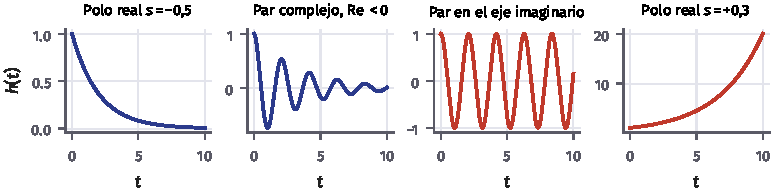
\includegraphics[width=0.95\linewidth]{polos_estabilidad_s}
  \caption{Posición de los polos en el plano $s$ y forma del modo correspondiente.}
\end{figure}

\begin{ejemplo}{Circuito RC}{rc}
  En un circuito RC paso bajo, con la entrada $x$ aplicada a la serie y la salida $y$ tomada en el condensador, $RC\,\dv{y}{t}+y=x$. Transformando,
  \[
    H(s)=\frac{1}{1+RCs},
  \]
  con un único polo en $s=-1/RC$: el sistema es causal y estable. Su respuesta al impulso es $h(t)=\frac{1}{RC}\e^{-t/RC}u(t)$ y su respuesta al escalón, $s(t)=\big(1-\e^{-t/RC}\big)u(t)$, que alcanza el 63\,\% del valor final en $t=RC$. La respuesta en frecuencia,
  \[
    \abs{H(j\omega)}=\frac{1}{\sqrt{1+(\omega RC)^2}},
  \]
  es la de un paso bajo con frecuencia de corte $\omega_c=1/RC$, donde la ganancia cae $3$\,dB. Con $R=\SI{1}{\kilo\ohm}$ y $C=\SI{1}{\micro\farad}$, $RC=\SI{1}{\milli\second}$, el polo está en $-1000$ y la frecuencia de corte es \SI{1000}{\radian\per\second}, unos \SI{159}{\hertz}.
  \begin{center}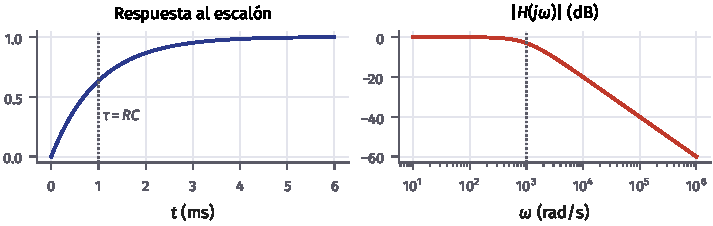
\includegraphics[width=0.6\linewidth]{rc_respuestas}\end{center}
\end{ejemplo}

\begin{encodigo}
  \codigo{lti_continuo}
\end{encodigo}

\subsection{Sistemas discretos: ecuación en diferencias y función de transferencia}

Los sistemas LTI discretos de orden finito se describen con una ecuación en diferencias. La forma estándar, que es la que usan \texttt{filter} en Matlab y \texttt{scipy.signal.lfilter} en Python, normaliza $a_0=1$:
\[
  \sum_{k=0}^{N}a_k\,y[n-k]=\sum_{k=0}^{M}b_k\,x[n-k]
  \quad\overset{\Zt}{\longrightarrow}\quad
  H(z)=\frac{\sum_{k=0}^{M}b_k\,z^{-k}}{1+\sum_{k=1}^{N}a_k\,z^{-k}}.
\]
A diferencia de la ecuación diferencial, la ecuación en diferencias es directamente un algoritmo. Despejando $y[n]$,
\[
  y[n]=\sum_{k=0}^{M}b_k\,x[n-k]-\sum_{k=1}^{N}a_k\,y[n-k],
\]
cada muestra de la salida se calcula a partir de las entradas actual y anteriores y de las salidas anteriores: es un cálculo \emph{recursivo}. Si la ecuación se escribe con adelantos, $\sum a_k\,y[n+k]=\sum b_k\,x[n+k]$, se llega a la misma $H(z)$ en potencias positivas de $z$; basta multiplicar numerador y denominador por $z^{-N}$ para pasar de una forma a otra.

\begin{importante}[Estabilidad de un sistema discreto causal]
  Un sistema causal con $H(z)$ racional es estable si y solo si todos sus polos están dentro de la circunferencia unidad: $\abs{p_i}<1$. Equivale a que la ROC, $\abs{z}>\max\abs{p_i}$, contenga la circunferencia unidad.
\end{importante}

El razonamiento es el mismo que en continuo: cada polo $p$ aporta a $h[n]$ un modo $p^nu[n]$, que decae si $\abs{p}<1$, se mantiene si $\abs{p}=1$ y crece si $\abs{p}>1$. Un par $r\e^{\pm j\Omega_0}$ aporta $r^n\cos(\Omega_0n+\phi)$, y un polo real negativo da una respuesta que alterna de signo.

\begin{figure}[ht]
  \centering
  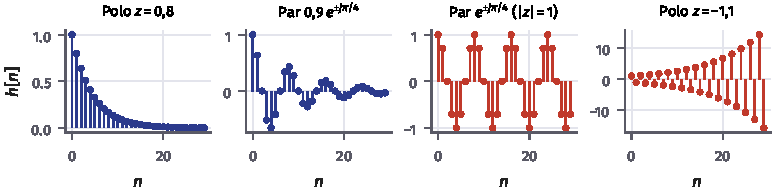
\includegraphics[width=0.95\linewidth]{polos_estabilidad_z}
  \caption{Posición de los polos en el plano $z$ y forma del modo correspondiente.}
\end{figure}

\begin{ejemplo}{Suavizado exponencial}{suavizado}
  El sistema $y[n]=0{,}8\,y[n-1]+0{,}2\,x[n]$ tiene, en forma estándar, $b=[0{,}2]$ y $a=[1,\,-0{,}8]$, y por tanto
  \[
    H(z)=\frac{0{,}2}{1-0{,}8z^{-1}},\qquad h[n]=0{,}2\,(0{,}8)^nu[n].
  \]
  Su único polo, $z=0{,}8$, está dentro de la circunferencia unidad: es estable. Lo confirma la condición sobre $h$: $\sum_n\abs{h[n]}=0{,}2/(1-0{,}8)=1$. La ganancia en continua es $H(1)=1$, de modo que una entrada constante sale sin cambios, y la respuesta en frecuencia es la del ejemplo~\ref{ej:sinusoide}.
\end{ejemplo}

\begin{encodigo}
  Convenio de \texttt{filter}/\texttt{lfilter}: \texttt{b} son los coeficientes de $x[n-k]$ y \texttt{a} los de $y[n-k]$, con \texttt{a[0]=1}.
  \codigo{lti_discreto}
\end{encodigo}

\subsection{Sistemas FIR e IIR}

Si todos los $a_k$ con $k\ge1$ son nulos, el sistema no es recursivo:
\[
  y[n]=\sum_{k=0}^{M}b_k\,x[n-k],\qquad h[n]=\begin{cases}b_n & 0\le n\le M\\0 & \text{en otro caso.}\end{cases}
\]
Su respuesta al impulso tiene $M+1$ muestras: es un sistema de \emph{respuesta al impulso finita} (FIR). Todos sus polos están en $z=0$ y, como $\sum\abs{h[n]}$ es una suma finita, es \emph{siempre estable}. Además, si sus coeficientes son simétricos, tiene fase lineal (Tema~4). Si algún $a_k$ con $k\ge1$ es distinto de cero, el sistema es recursivo y, en general, su respuesta al impulso tiene duración infinita: es un sistema IIR. Un IIR puede ser inestable, por lo que hay que comprobar sus polos, pero a cambio consigue la misma selectividad que un FIR con muchos menos coeficientes.

\begin{ejemplo}{Media móvil y suavizado exponencial}{fir-iir}
  La media móvil de cinco muestras, $y[n]=\frac15\sum_{k=0}^{4}x[n-k]$, es un FIR con $h[n]=\frac15$ para $0\le n\le4$. El suavizado exponencial del ejemplo~\ref{ej:suavizado} es un IIR con un solo coeficiente de realimentación. Los dos suavizan la señal, pero el IIR «recuerda» todo el pasado con un peso que decae exponencialmente.
  \begin{center}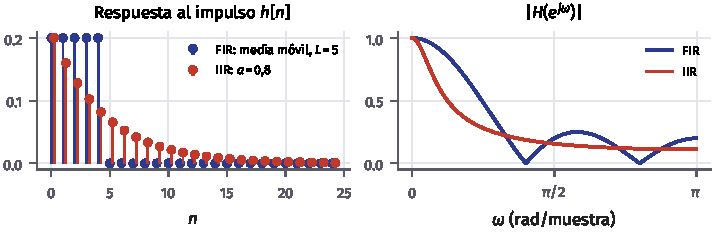
\includegraphics[width=0.6\linewidth]{fir_iir}\end{center}
\end{ejemplo}

\paragraph{Diagramas de bloques.} Con sumadores, multiplicadores por constantes y retardos de una muestra ($z^{-1}$) se implementa cualquier ecuación en diferencias, y eso es lo que ejecuta un DSP o un microcontrolador. Un FIR es una línea de retardos cuyas salidas se ponderan con los $b_k$ y se suman; un IIR añade un lazo que realimenta las salidas anteriores ponderadas con $-a_k$ (\cref{fig:bloques}).

\begin{figure}[ht]
  \centering
  \begin{tikzpicture}[every node/.style={font=\small}]
    \node (x) at (0,0) {$x[n]$};
    \node[bloque, minimum width=9mm] (d1) at (2,0) {$z^{-1}$};
    \node[bloque, minimum width=9mm] (d2) at (4,0) {$z^{-1}$};
    \node[sumador] (s1) at (3,-1.6) {$+$};
    \node[sumador] (s2) at (5,-1.6) {$+$};
    \draw[flecha] (x) -- (d1); \draw[flecha] (d1) -- (d2);
    \draw[thick, pdsgris] (d2) -- (5,0);
    \draw[flecha] (1,0) -- node[left]{$b_0$} (1,-1.6) -- (s1);
    \draw[flecha] (3,0) -- node[right]{$b_1$} (s1);
    \draw[flecha] (5,0) -- node[right]{$b_2$} (s2);
    \draw[flecha] (s1) -- (s2);
    \draw[flecha] (s2) -- (6.2,-1.6) node[right]{$y[n]$};
    \fill[pdsgris] (1,0) circle (1.2pt) (3,0) circle (1.2pt);
  \end{tikzpicture}\hspace{1.2cm}
  \begin{tikzpicture}[node distance=0.6cm and 0.8cm, every node/.style={font=\small}]
    \node (x) {$x[n]$};
    \node[bloque, minimum width=9mm, right=of x] (b0) {$b_0$};
    \node[sumador, right=of b0] (s) {$+$};
    \coordinate[right=0.8cm of s] (c);
    \node[right=0.4cm of c] (y) {$y[n]$};
    \node[bloque, minimum width=9mm, below=0.6cm of c] (d) {$z^{-1}$};
    \node[bloque, minimum width=9mm, left=0.5cm of d] (a1) {$-a_1$};
    \draw[flecha] (x) -- (b0); \draw[flecha] (b0) -- (s); \draw[thick, pdsgris] (s) -- (c);
    \draw[flecha] (c) -- (y);
    \draw[flecha] (c) -- (d); \draw[flecha] (d) -- (a1); \draw[flecha] (a1) -| (s);
  \end{tikzpicture}
  \caption{Diagramas de bloques de un FIR de orden 2, $y[n]=b_0x[n]+b_1x[n-1]+b_2x[n-2]$, y de un IIR de primer orden, $y[n]=b_0x[n]-a_1y[n-1]$.}
  \label{fig:bloques}
\end{figure}

\paragraph{¿Hay sistemas FIR en tiempo continuo?} Un sistema continuo descrito por una ecuación diferencial de orden finito tiene $H(s)$ racional y su $h(t)$ es una suma de modos $\e^{p_it}u(t)$, de duración infinita (más, si $M\ge N$, términos con $\delta$ y sus derivadas). Existen sistemas continuos con respuesta al impulso de duración finita, como el integrador de ventana
\[
  y(t)=\int_{t-T}^{t}x(\tau)\dd\tau,\qquad h(t)=u(t)-u(t-T),\qquad H(s)=\frac{1-\e^{-sT}}{s},
\]
pero su función de transferencia no es racional y no se puede construir con un número finito de resistencias, condensadores y bobinas; solo se aproxima. En discreto, en cambio, un FIR es trivial: basta una línea de retardos. Es una de las ventajas del procesado digital, porque los FIR, siempre estables y con fase lineal posible, solo son prácticos en tiempo discreto.

\begin{flushright}\small\color{pdsgris}Ejercicios 11–16. \herramienta{T1-respuesta-lti-continua, T1-respuesta-lti-discreta}.\end{flushright}

% =====================================================================
\section{Contenido en frecuencia de señales reales}\label{sec:aplicaciones}

Cada tipo de señal ocupa una banda de frecuencias característica, y cada fuente de ruido o interferencia también. Conocer las dos bandas decide casi todo el diseño de un sistema de procesado: la frecuencia de muestreo mínima ($f_s>2f_{\max}$, Tema~2), el filtro que separa la señal del ruido (Tema~4) y la resolución en frecuencia que hace falta para analizarla (Tema~3). La \cref{fig:bandas} resume, en escala logarítmica, las bandas de las aplicaciones que se comentan a continuación, desde las centésimas de hercio de la sismología hasta los cientos de terahercios de la fibra óptica.

\begin{figure}[ht]
  \centering
  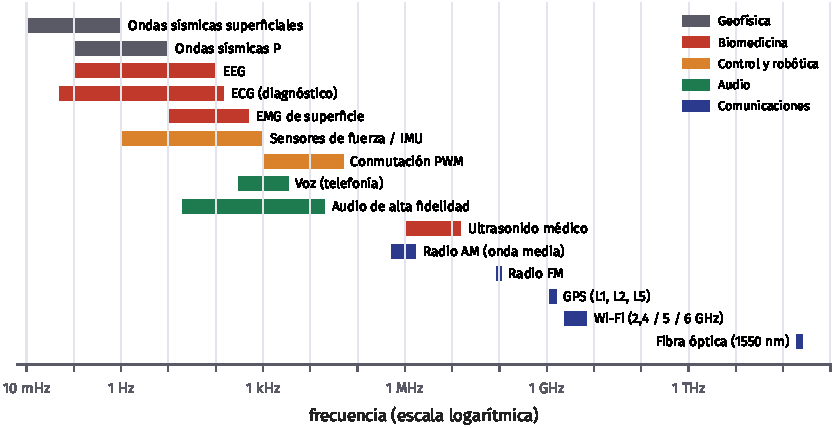
\includegraphics[width=0.85\linewidth]{bandas_aplicaciones}
  \caption{Bandas de frecuencia de algunas aplicaciones (escala logarítmica).}
  \label{fig:bandas}
\end{figure}

\paragraph{Comunicaciones.} La voz en telefonía ocupa de \SI{300}{\hertz} a \SI{3,4}{\kilo\hertz}; la radio AM de onda media, de \SI{526,5}{\kilo\hertz} a \SI{1606,5}{\kilo\hertz}; la FM, de \SI{87,5}{\mega\hertz} a \SI{108}{\mega\hertz}; el GPS usa la banda L1 (\SI{1575,42}{\mega\hertz}), además de L2 y L5; el Wi-Fi, las bandas de \SI{2,4}{}, \SI{5}{} y \SI{6}{\giga\hertz}; y la fibra óptica, luz de \SI{1550}{\nano\metre}, unos \SI{193}{\tera\hertz}. El ruido térmico es blanco: se reparte por igual en toda la banda y su potencia crece con el ancho de banda del receptor ($kTB$). Hay además interferencias electromagnéticas de otros equipos y desvanecimientos por multitrayecto, variaciones lentas de la amplitud que van de hercios a kilohercios según la velocidad del receptor. Las señales de radio se procesan casi siempre en banda base, después de desplazarlas en frecuencia con la propiedad de modulación de la transformada de Fourier.

\paragraph{Audio y música.} La banda audible va de \SI{20}{\hertz} a \SI{20}{\kilo\hertz} y se suele dividir en subgraves (20–60\,Hz), graves (60–250\,Hz), medios (250\,Hz–2\,kHz) y agudos (2–20\,kHz). Las frecuencias de muestreo habituales son \SI{8}{\kilo\hertz} en telefonía, \SI{44,1}{\kilo\hertz} en el CD, \SI{48}{\kilo\hertz} en vídeo y 96 o \SI{192}{\kilo\hertz} en estudio. El ruido de cuantificación es aproximadamente blanco, repartido en toda la banda $[0,f_s/2]$, con potencia $\Delta^2/12$ (Tema~2). La red eléctrica induce un zumbido de \SI{50}{\hertz} en Europa (\SI{60}{\hertz} en América) y sus armónicos; el ruido ambiental es de banda ancha y los clics y chasquidos son impulsivos. El proyecto «Audio con ruido» trabaja con una grabación que contiene los cuatro tipos de ruido: el zumbido se elimina con filtros de muesca o en peine, el soplido de banda ancha con un paso bajo o un filtro de Wiener, los clics con predicción lineal y un silbido de frecuencia variable con la STFT.

\paragraph{Señales biomédicas.} El ECG ocupa de \SI{0,05}{\hertz} a \SI{150}{\hertz} en diagnóstico (de \SI{0,5}{\hertz} a \SI{40}{\hertz} en monitorización); el EEG, de \SI{0,5}{\hertz} a \SI{100}{\hertz}, con los ritmos delta (0,5–4\,Hz), theta (4–8\,Hz), alfa (8–13\,Hz), beta (13–30\,Hz) y gamma (más de 30\,Hz); el EMG de superficie, de \SI{10}{\hertz} a \SI{500}{\hertz}; el fonocardiograma, de \SI{20}{\hertz} a \SI{1}{\kilo\hertz}, aproximadamente; y la ecografía usa ultrasonidos de 2 a \SI{15}{\mega\hertz}. Las perturbaciones típicas son la red eléctrica (50/60\,Hz), la deriva de la línea base por la respiración (por debajo de \SI{0,5}{\hertz}), los artefactos de movimiento (por debajo de \SI{10}{\hertz}) y la actividad muscular superpuesta al ECG (por encima de \SI{20}{\hertz}). Como se ve, las bandas de la señal y del ruido se solapan, y eso es lo que hace difícil el problema. El proyecto «ECG» parte de registros de holter muestreados a \SI{360}{\hertz} con deriva, red, ruido muscular y artefactos: hay que limpiarlos sin deformar el segmento ST, detectar los latidos con el algoritmo de Pan-Tompkins y analizar la variabilidad del ritmo.

\paragraph{Control y robótica.} Las señales de posición, velocidad, fuerza o de una IMU tienen su dinámica útil por debajo de 0,1–1\,kHz. Una cámara a 30–60 fotogramas por segundo solo puede representar variaciones de hasta 15–30\,Hz, la mitad de su frecuencia de muestreo. En un LiDAR la luz es óptica (905 o \SI{1550}{\nano\metre}), pero lo que marca el muestreo de la escena es la \emph{tasa de barrido}, de \SI{10}{\hertz} a \SI{1}{\kilo\hertz}. La conmutación PWM de los motores está entre 1 y \SI{50}{\kilo\hertz}, y los buses de comunicación van de \SI{125}{\kilo\bit\per\second} a \SI{1}{\mega\bit\per\second} en CAN o a \SI{100}{\mega\bit\per\second} en EtherCAT. El ruido incluye la deriva térmica y el ruido $1/f$ de los sensores (de baja frecuencia), el ruido térmico y el de cuantificación (blancos) y las vibraciones y resonancias mecánicas (de \SI{10}{\hertz} a \SI{10}{\kilo\hertz}). El proyecto «Registro de carrera» usa sesiones reales con velocidad GPS, frecuencia cardiaca y altitud, muestreadas de forma irregular: hay que remuestrearlas, filtrarlas, modelar el ruido y detectar los cambios de ritmo.

\paragraph{Geofísica y sismología.} Las ondas sísmicas P tienen frecuencias de 0,1 a \SI{10}{\hertz} y las S, de 0,1 a \SI{3}{\hertz}; las ondas superficiales (Rayleigh y Love), que son las que más dañan las estructuras, de 0,01 a \SI{1}{\hertz}. Los microtremores están entre 0,1 y \SI{1}{\hertz} y las vibraciones de estructuras entre 0,1 y \SI{100}{\hertz}, donde interesan sobre todo sus resonancias. El ruido procede de la actividad humana (tráfico, maquinaria: de 1 a \SI{10}{\hertz} y más), de los microsismos del oleaje (0,1–0,3\,Hz) y del viento y la presión atmosférica (por debajo de \SI{1}{\hertz}). Con señales de tan baja frecuencia, lo que limita la resolución espectral no es la frecuencia de muestreo sino la duración del registro: $\Delta f\approx1/T_{\mathrm{obs}}$ (Tema~3).

\paragraph{Imagen.} En una imagen la variable independiente es espacial y la frecuencia se mide en ciclos por píxel o por milímetro. Las bajas frecuencias corresponden a las zonas uniformes y las altas, a los bordes, las texturas y el ruido. Los ruidos típicos son el gaussiano del sensor (de banda ancha), el de sal y pimienta (impulsivo) y los patrones periódicos, que aparecen como picos aislados en el espectro bidimensional. Los proyectos «Imagen con ruido» y «Códigos de barras» restauran imágenes con estos defectos y con desenfoque, y leen códigos EAN-13 tratando cada fila de la imagen como una señal unidimensional muestreada.

\begin{nota}[En resumen]
  El ruido térmico y el de cuantificación son de banda ancha; la interferencia de la red eléctrica es de banda estrecha (50/60\,Hz y armónicos); las derivas son de muy baja frecuencia. La banda de la señal fija la frecuencia de muestreo y el tipo de filtro. Los proyectos de evaluación del curso trabajan sobre estas situaciones.
\end{nota}

% =====================================================================
\section*{Resumen del tema}
\addcontentsline{toc}{section}{Resumen del tema}

\begin{itemize}
  \item Señal y sistema; notación $x(t)$ frente a $x[n]$, $\omega$ frente a $\Omega$.
  \item Clasificación de señales: analógica, muestreada, digital; determinista o aleatoria; periódica (con su periodo fundamental); par o impar; causal; de energía o de potencia; real, compleja o hermítica.
  \item Señales básicas: $\delta$, $u$, $r$, $\rect$, $\tri$, $\sinc$, $\sgn$ y exponenciales. La exponencial discreta $\e^{j\Omega_0n}$ solo es periódica si $\Omega_0/2\pi$ es racional, y $\Omega_0$ y $\Omega_0+2\pi$ dan la misma secuencia.
  \item Operaciones sobre la variable independiente (desplazar primero, escalar después) y sobre la amplitud; diferencia y acumulación como análogos de la derivada y la integral.
  \item Convolución: definición, cálculo gráfico, propiedades y longitud del resultado.
  \item Series de Fourier continua y discreta, CTFT y DTFT (periódica de periodo $2\pi$). Convolución en el tiempo $\leftrightarrow$ producto en frecuencia.
  \item Laplace y Z bilaterales, siempre con su región de convergencia.
  \item Propiedades de los sistemas: memoria, causalidad, estabilidad BIBO, invertibilidad, linealidad e invarianza temporal.
  \item Un sistema LTI queda caracterizado por $h$: $y=x\conv h$; causalidad y estabilidad se leen en $h$ y en los polos.
  \item Las exponenciales son autofunciones: $\e^{j\omega t}\to H(j\omega)\,\e^{j\omega t}$.
  \item Ecuaciones diferenciales y en diferencias, función de transferencia, polos, ceros y estabilidad; sistemas FIR e IIR.
\end{itemize}

% =====================================================================
\section*{Bibliografía}
\addcontentsline{toc}{section}{Bibliografía}

\begin{itemize}
  \item F.~T. Ulaby y A.~E. Yagle, \emph{Signals and Systems: Theory and Applications}, 2.ª ed. Michigan Publishing Services, 2024. Capítulos 1 y 2. Descarga libre en \url{https://services.publishing.umich.edu/Books/S/Signals-and-Systems}.
  \item A.~V. Oppenheim y A.~S. Willsky, \emph{Señales y sistemas}, 2.ª ed. Prentice Hall, 1997. Capítulos 1 a 5, 9 y 10. Es la referencia clásica para todo el tema.
  \item J.~G. Proakis y D.~G. Manolakis, \emph{Tratamiento digital de señales}, 4.ª ed. Pearson Prentice Hall, 2007. Capítulos 1 a 4, para la parte discreta.
  \item V.~K. Ingle y J.~G. Proakis, \emph{Digital Signal Processing Using MATLAB}, 3.ª ed. Cengage Learning, 2012. Capítulos 2 a 4, con ejemplos en Matlab.
\end{itemize}

\end{document}
